\documentclass[11pt,letterpaper,]{article}
\usepackage{lmodern}
\usepackage{amssymb,amsmath}
\usepackage{ifxetex,ifluatex}
\usepackage{fixltx2e} % provides \textsubscript
\ifnum 0\ifxetex 1\fi\ifluatex 1\fi=0 % if pdftex
  \usepackage[T1]{fontenc}
  \usepackage[utf8]{inputenc}
\else % if luatex or xelatex
  \ifxetex
    \usepackage{mathspec}
  \else
    \usepackage{fontspec}
  \fi
  \defaultfontfeatures{Ligatures=TeX,Scale=MatchLowercase}
\fi
% use upquote if available, for straight quotes in verbatim environments
\IfFileExists{upquote.sty}{\usepackage{upquote}}{}
% use microtype if available
\IfFileExists{microtype.sty}{%
\usepackage{microtype}
\UseMicrotypeSet[protrusion]{basicmath} % disable protrusion for tt fonts
}{}
\usepackage[margin=1in]{geometry}
\usepackage{hyperref}
\hypersetup{unicode=true,
            pdftitle={Global Terrorism},
            pdfauthor={Group Four; Tom Kennon, Adam Busa, Asa Brigandi, Jiapeng Guo},
            pdfborder={0 0 0},
            breaklinks=true}
\urlstyle{same}  % don't use monospace font for urls
\usepackage{natbib}
\bibliographystyle{datalab}
\usepackage{color}
\usepackage{fancyvrb}
\newcommand{\VerbBar}{|}
\newcommand{\VERB}{\Verb[commandchars=\\\{\}]}
\DefineVerbatimEnvironment{Highlighting}{Verbatim}{commandchars=\\\{\}}
% Add ',fontsize=\small' for more characters per line
\usepackage{framed}
\definecolor{shadecolor}{RGB}{248,248,248}
\newenvironment{Shaded}{\begin{snugshade}}{\end{snugshade}}
\newcommand{\KeywordTok}[1]{\textcolor[rgb]{0.13,0.29,0.53}{\textbf{{#1}}}}
\newcommand{\DataTypeTok}[1]{\textcolor[rgb]{0.13,0.29,0.53}{{#1}}}
\newcommand{\DecValTok}[1]{\textcolor[rgb]{0.00,0.00,0.81}{{#1}}}
\newcommand{\BaseNTok}[1]{\textcolor[rgb]{0.00,0.00,0.81}{{#1}}}
\newcommand{\FloatTok}[1]{\textcolor[rgb]{0.00,0.00,0.81}{{#1}}}
\newcommand{\ConstantTok}[1]{\textcolor[rgb]{0.00,0.00,0.00}{{#1}}}
\newcommand{\CharTok}[1]{\textcolor[rgb]{0.31,0.60,0.02}{{#1}}}
\newcommand{\SpecialCharTok}[1]{\textcolor[rgb]{0.00,0.00,0.00}{{#1}}}
\newcommand{\StringTok}[1]{\textcolor[rgb]{0.31,0.60,0.02}{{#1}}}
\newcommand{\VerbatimStringTok}[1]{\textcolor[rgb]{0.31,0.60,0.02}{{#1}}}
\newcommand{\SpecialStringTok}[1]{\textcolor[rgb]{0.31,0.60,0.02}{{#1}}}
\newcommand{\ImportTok}[1]{{#1}}
\newcommand{\CommentTok}[1]{\textcolor[rgb]{0.56,0.35,0.01}{\textit{{#1}}}}
\newcommand{\DocumentationTok}[1]{\textcolor[rgb]{0.56,0.35,0.01}{\textbf{\textit{{#1}}}}}
\newcommand{\AnnotationTok}[1]{\textcolor[rgb]{0.56,0.35,0.01}{\textbf{\textit{{#1}}}}}
\newcommand{\CommentVarTok}[1]{\textcolor[rgb]{0.56,0.35,0.01}{\textbf{\textit{{#1}}}}}
\newcommand{\OtherTok}[1]{\textcolor[rgb]{0.56,0.35,0.01}{{#1}}}
\newcommand{\FunctionTok}[1]{\textcolor[rgb]{0.00,0.00,0.00}{{#1}}}
\newcommand{\VariableTok}[1]{\textcolor[rgb]{0.00,0.00,0.00}{{#1}}}
\newcommand{\ControlFlowTok}[1]{\textcolor[rgb]{0.13,0.29,0.53}{\textbf{{#1}}}}
\newcommand{\OperatorTok}[1]{\textcolor[rgb]{0.81,0.36,0.00}{\textbf{{#1}}}}
\newcommand{\BuiltInTok}[1]{{#1}}
\newcommand{\ExtensionTok}[1]{{#1}}
\newcommand{\PreprocessorTok}[1]{\textcolor[rgb]{0.56,0.35,0.01}{\textit{{#1}}}}
\newcommand{\AttributeTok}[1]{\textcolor[rgb]{0.77,0.63,0.00}{{#1}}}
\newcommand{\RegionMarkerTok}[1]{{#1}}
\newcommand{\InformationTok}[1]{\textcolor[rgb]{0.56,0.35,0.01}{\textbf{\textit{{#1}}}}}
\newcommand{\WarningTok}[1]{\textcolor[rgb]{0.56,0.35,0.01}{\textbf{\textit{{#1}}}}}
\newcommand{\AlertTok}[1]{\textcolor[rgb]{0.94,0.16,0.16}{{#1}}}
\newcommand{\ErrorTok}[1]{\textcolor[rgb]{0.64,0.00,0.00}{\textbf{{#1}}}}
\newcommand{\NormalTok}[1]{{#1}}
\usepackage{longtable,booktabs}
\usepackage{graphicx,grffile}
\makeatletter
\def\maxwidth{\ifdim\Gin@nat@width>\linewidth\linewidth\else\Gin@nat@width\fi}
\def\maxheight{\ifdim\Gin@nat@height>\textheight\textheight\else\Gin@nat@height\fi}
\makeatother
% Scale images if necessary, so that they will not overflow the page
% margins by default, and it is still possible to overwrite the defaults
% using explicit options in \includegraphics[width, height, ...]{}
\setkeys{Gin}{width=\maxwidth,height=\maxheight,keepaspectratio}
\IfFileExists{parskip.sty}{%
\usepackage{parskip}
}{% else
\setlength{\parindent}{0pt}
\setlength{\parskip}{6pt plus 2pt minus 1pt}
}
\setlength{\emergencystretch}{3em}  % prevent overfull lines
\providecommand{\tightlist}{%
  \setlength{\itemsep}{0pt}\setlength{\parskip}{0pt}}
\setcounter{secnumdepth}{5}
% Redefines (sub)paragraphs to behave more like sections
\ifx\paragraph\undefined\else
\let\oldparagraph\paragraph
\renewcommand{\paragraph}[1]{\oldparagraph{#1}\mbox{}}
\fi
\ifx\subparagraph\undefined\else
\let\oldsubparagraph\subparagraph
\renewcommand{\subparagraph}[1]{\oldsubparagraph{#1}\mbox{}}
\fi

%%% Use protect on footnotes to avoid problems with footnotes in titles
\let\rmarkdownfootnote\footnote%
\def\footnote{\protect\rmarkdownfootnote}

%%% Change title format to be more compact
\usepackage{titling}

% Create subtitle command for use in maketitle
\newcommand{\subtitle}[1]{
  \posttitle{
    \begin{center}\large#1\end{center}
    }
}

\setlength{\droptitle}{-2em}
  \title{Global Terrorism}
  \pretitle{\vspace{\droptitle}\centering\huge}
  \posttitle{\par}
\subtitle{STAT 4185 Project Final}
  \author{Group Four; Tom Kennon, Adam Busa, Asa Brigandi, Jiapeng Guo}
  \preauthor{\centering\large\emph}
  \postauthor{\par}
  \predate{\centering\large\emph}
  \postdate{\par}
  \date{28 April 2018}


\usepackage{amsthm}
\newtheorem{theorem}{Theorem}[section]
\newtheorem{lemma}{Lemma}[section]
\theoremstyle{definition}
\newtheorem{definition}{Definition}[section]
\newtheorem{corollary}{Corollary}[section]
\newtheorem{proposition}{Proposition}[section]
\theoremstyle{definition}
\newtheorem{example}{Example}[section]
\theoremstyle{definition}
\newtheorem{exercise}{Exercise}[section]
\theoremstyle{remark}
\newtheorem*{remark}{Remark}
\newtheorem*{solution}{Solution}
\begin{document}
\maketitle

{
\setcounter{tocdepth}{3}
\tableofcontents
}
\newpage

\section{Introduction}\label{sec:intro}

Our project is focused on analyzing global terrorism data. With many
terrorist attacks prevalent in the news since the early 2000s as well as
imposing threats of attacks being a controversial topic for a newly
elected president, this an important topic at the forefront of people's
minds. The data source we used for our analysis is The Global Terrorism
Database (GTD) which is an open source database that contains
information about specific global terrorism incidents spanning from 1970
to 2016. The dataset is available at:
\url{https://www.kaggle.com/START-UMD/gtd}. The total dataset contains
170,350 records with 135 variables. Each record contains the date of
incident, location of the incident, information about the target,
information about the perpetrators etc. Some of the variables are
repetitive, do not tell provide much insight for the data, and/or are
riddled with missing values as this is a real-world dataset.

Some of exploratory questions we set out to accomplish in this project
are:

\begin{itemize}
\tightlist
\item
  What are the factors (possibly weapon type, attack type, HDI, etc.)
  that predict the terrorist group that perpetrated an attack?
\item
  Investigate the trends in mass terrorism (terrorist attacks with many
  people killed) in the dataset. Identify any possible unique
  characteristics of mass terrorism.
\item
  What factors may predict the success rate of attacks? What are the
  significant drivers for a terrorist attack to be ``successful''? Is
  there a bias pertaining to the recency of an attack? {[}Some possible
  solutions: logit/probit prediction, random forest model{]}
\end{itemize}

\section{Data Wrangling}\label{sec:data_wrangling}

The first step to any data science project is to read in the data. Here
is the global terrorism dataset that we called: ``gt'' provided in a
tibble format to improve readability in its data structure.

\begin{Shaded}
\begin{Highlighting}[]
\NormalTok{## Reads in data}
\NormalTok{gt <-}\StringTok{ }\KeywordTok{read.csv}\NormalTok{(}\StringTok{"globalterrorismdb_0617dist.csv"}\NormalTok{)}

\KeywordTok{library}\NormalTok{(tidyverse)}

\KeywordTok{library}\NormalTok{(knitr)}

\NormalTok{## Shows dataset structure}
\KeywordTok{as_tibble}\NormalTok{(gt)}
\end{Highlighting}
\end{Shaded}

\begin{verbatim}
## # A tibble: 170,350 x 135
##         eventid iyear imonth  iday approxdate extended resolution country
##           <dbl> <int>  <int> <int> <fct>         <int> <fct>        <int>
##  1 197000000001  1970      7     2 ""                0 ""              58
##  2 197000000002  1970      0     0 ""                0 ""             130
##  3 197001000001  1970      1     0 ""                0 ""             160
##  4 197001000002  1970      1     0 ""                0 ""              78
##  5 197001000003  1970      1     0 ""                0 ""             101
##  6 197001010002  1970      1     1 ""                0 ""             217
##  7 197001020001  1970      1     2 ""                0 ""             218
##  8 197001020002  1970      1     2 ""                0 ""             217
##  9 197001020003  1970      1     2 ""                0 ""             217
## 10 197001030001  1970      1     3 ""                0 ""             217
## # ... with 170,340 more rows, and 127 more variables: country_txt <fct>,
## #   region <int>, region_txt <fct>, provstate <fct>, city <fct>,
## #   latitude <dbl>, longitude <dbl>, specificity <int>, vicinity <int>,
## #   location <fct>, summary <fct>, crit1 <int>, crit2 <int>, crit3 <int>,
## #   doubtterr <int>, alternative <int>, alternative_txt <fct>,
## #   multiple <int>, success <int>, suicide <int>, attacktype1 <int>,
## #   attacktype1_txt <fct>, attacktype2 <int>, attacktype2_txt <fct>,
## #   attacktype3 <int>, attacktype3_txt <fct>, targtype1 <int>,
## #   targtype1_txt <fct>, targsubtype1 <int>, targsubtype1_txt <fct>,
## #   corp1 <fct>, target1 <fct>, natlty1 <int>, natlty1_txt <fct>,
## #   targtype2 <int>, targtype2_txt <fct>, targsubtype2 <int>,
## #   targsubtype2_txt <fct>, corp2 <fct>, target2 <fct>, natlty2 <int>,
## #   natlty2_txt <fct>, targtype3 <int>, targtype3_txt <fct>,
## #   targsubtype3 <int>, targsubtype3_txt <fct>, corp3 <fct>,
## #   target3 <fct>, natlty3 <int>, natlty3_txt <fct>, gname <fct>,
## #   gsubname <fct>, gname2 <fct>, gsubname2 <fct>, gname3 <fct>,
## #   gsubname3 <fct>, motive <fct>, guncertain1 <int>, guncertain2 <int>,
## #   guncertain3 <int>, individual <int>, nperps <int>, nperpcap <dbl>,
## #   claimed <int>, claimmode <int>, claimmode_txt <fct>, claim2 <int>,
## #   claimmode2 <int>, claimmode2_txt <fct>, claim3 <int>,
## #   claimmode3 <int>, claimmode3_txt <fct>, compclaim <int>,
## #   weaptype1 <int>, weaptype1_txt <fct>, weapsubtype1 <int>,
## #   weapsubtype1_txt <fct>, weaptype2 <int>, weaptype2_txt <fct>,
## #   weapsubtype2 <int>, weapsubtype2_txt <fct>, weaptype3 <int>,
## #   weaptype3_txt <fct>, weapsubtype3 <int>, weapsubtype3_txt <fct>,
## #   weaptype4 <int>, weaptype4_txt <fct>, weapsubtype4 <int>,
## #   weapsubtype4_txt <fct>, weapdetail <fct>, nkill <int>, nkillus <int>,
## #   nkillter <int>, nwound <int>, nwoundus <int>, nwoundte <int>,
## #   property <int>, propextent <int>, propextent_txt <fct>,
## #   propvalue <dbl>, ...
\end{verbatim}

It is often useful to include external datasets to highlight insights
that may have even been unknown beforehand with just the first dataset
as reference. Our first helpful dataset is a simple gross count of total
world population for each year in the dataset 1960-2016. This is helpful
for getting a better understanding of per capita statistics for each
year rather than only total numbers for each year. The second external
dataset we found helpful was a Gross Domestic Product (GDP) dataset for
each country in the world. We have added the GDP of the target country
from the incident year into our main dataset. The GDP data was taken
from the World Bank database. We believe that GDP may be an important
tool for predicting terrorist attacks. Both of these dataset's
structures are shown in tibble format below.

\begin{Shaded}
\begin{Highlighting}[]
\KeywordTok{library}\NormalTok{(}\StringTok{"readxl"}\NormalTok{)}

\NormalTok{## Reads in data}
\NormalTok{popworld <-}\StringTok{ }\KeywordTok{read_excel}\NormalTok{(}\StringTok{"world population.xlsx"}\NormalTok{)}

\NormalTok{## Shows dataset structure}
\KeywordTok{as_tibble}\NormalTok{(popworld)}
\end{Highlighting}
\end{Shaded}

\begin{verbatim}
## # A tibble: 57 x 2
##    population  year
##         <dbl> <dbl>
##  1 3034193297  1960
##  2 3075115342  1961
##  3 3127961482  1962
##  4 3192794384  1963
##  5 3258201476  1964
##  6 3324951621  1965
##  7 3394864530  1966
##  8 3464439525  1967
##  9 3534821115  1968
## 10 3609383725  1969
## # ... with 47 more rows
\end{verbatim}

\begin{Shaded}
\begin{Highlighting}[]
\NormalTok{## Reads in data}
\NormalTok{gdp<-}\KeywordTok{read.csv}\NormalTok{(}\StringTok{"GDP1.csv"}\NormalTok{, }\DataTypeTok{check.names =} \OtherTok{FALSE}\NormalTok{)}

\NormalTok{## Shows dataset structure}
\KeywordTok{as_tibble}\NormalTok{(gdp)}
\end{Highlighting}
\end{Shaded}

\begin{verbatim}
## # A tibble: 264 x 62
##    `Country Name` `Country Code` `Indicator Name` `Indicator Code`  `1960`
##    <fct>          <fct>          <fct>            <fct>              <dbl>
##  1 Aruba          ABW            GDP (current US~ NY.GDP.MKTP.CD   NA     
##  2 Afghanistan    AFG            GDP (current US~ NY.GDP.MKTP.CD    5.38e8
##  3 Angola         AGO            GDP (current US~ NY.GDP.MKTP.CD   NA     
##  4 Albania        ALB            GDP (current US~ NY.GDP.MKTP.CD   NA     
##  5 Andorra        AND            GDP (current US~ NY.GDP.MKTP.CD   NA     
##  6 Arab World     ARB            GDP (current US~ NY.GDP.MKTP.CD   NA     
##  7 United Arab E~ ARE            GDP (current US~ NY.GDP.MKTP.CD   NA     
##  8 Argentina      ARG            GDP (current US~ NY.GDP.MKTP.CD   NA     
##  9 Armenia        ARM            GDP (current US~ NY.GDP.MKTP.CD   NA     
## 10 American Samoa ASM            GDP (current US~ NY.GDP.MKTP.CD   NA     
## # ... with 254 more rows, and 57 more variables: `1961` <dbl>,
## #   `1962` <dbl>, `1963` <dbl>, `1964` <dbl>, `1965` <dbl>, `1966` <dbl>,
## #   `1967` <dbl>, `1968` <dbl>, `1969` <dbl>, `1970` <dbl>, `1971` <dbl>,
## #   `1972` <dbl>, `1973` <dbl>, `1974` <dbl>, `1975` <dbl>, `1976` <dbl>,
## #   `1977` <dbl>, `1978` <dbl>, `1979` <dbl>, `1980` <dbl>, `1981` <dbl>,
## #   `1982` <dbl>, `1983` <dbl>, `1984` <dbl>, `1985` <dbl>, `1986` <dbl>,
## #   `1987` <dbl>, `1988` <dbl>, `1989` <dbl>, `1990` <dbl>, `1991` <dbl>,
## #   `1992` <dbl>, `1993` <dbl>, `1994` <dbl>, `1995` <dbl>, `1996` <dbl>,
## #   `1997` <dbl>, `1998` <dbl>, `1999` <dbl>, `2000` <dbl>, `2001` <dbl>,
## #   `2002` <dbl>, `2003` <dbl>, `2004` <dbl>, `2005` <dbl>, `2006` <dbl>,
## #   `2007` <dbl>, `2008` <dbl>, `2009` <dbl>, `2010` <dbl>, `2011` <dbl>,
## #   `2012` <dbl>, `2013` <dbl>, `2014` <dbl>, `2015` <dbl>, `2016` <dbl>,
## #   `2017` <lgl>
\end{verbatim}

Now the next logical step in the data wrangling process is to join these
two datasets to the global terrorism dataset which we do in this next R
chunk. We also provided code with output that shows the merges were
successful. The sample\_n function is taking a random sample of 6 of the
events with their years and populations. The head function is showing
the first 6 events with their country and country's respective GDPs.

\begin{Shaded}
\begin{Highlighting}[]
\NormalTok{## Joins gt data and popworld data by year as "popworld2"}
\NormalTok{popworld2 <-}\StringTok{ }\KeywordTok{inner_join}\NormalTok{(popworld,gt,}\DataTypeTok{by=}\KeywordTok{c}\NormalTok{(}\StringTok{"year"}\NormalTok{=}\StringTok{"iyear"}\NormalTok{))}

\NormalTok{## Evidence that our join was successful}
\KeywordTok{set.seed}\NormalTok{(}\DecValTok{12345}\NormalTok{)}
\KeywordTok{sample_n}\NormalTok{(}\KeywordTok{select}\NormalTok{(popworld2, eventid, year, population),}\DecValTok{6}\NormalTok{)}
\end{Highlighting}
\end{Shaded}

\begin{verbatim}
## # A tibble: 6 x 3
##        eventid  year population
##          <dbl> <dbl>      <dbl>
## 1 201311030020  2013 7182860115
## 2 201506170047  2015 7355220412
## 3 201404050030  2014 7268986176
## 4 201507310083  2015 7355220412
## 5 200504090006  2005 6517020798
## 6 198606200001  1986 4928822143
\end{verbatim}

\begin{Shaded}
\begin{Highlighting}[]
\NormalTok{## Joins gt data and gdp data by country as "master"}
\NormalTok{## a bit more complicated because the gdp dataset was less straightforward than the popworld}
\KeywordTok{library}\NormalTok{(}\StringTok{"reshape2"}\NormalTok{)}
\NormalTok{gdp2<-}\KeywordTok{melt}\NormalTok{(gdp, }\DataTypeTok{id.vars =} \KeywordTok{c}\NormalTok{(}\StringTok{"Country Name"}\NormalTok{, }\StringTok{"Country Code"}\NormalTok{, }\StringTok{"Indicator Name"}\NormalTok{, }\StringTok{"Indicator Code"}\NormalTok{))}
\NormalTok{gdp3<-gdp2 %>%}\StringTok{ }\KeywordTok{select}\NormalTok{(}\StringTok{"Country Name"}\NormalTok{, }\StringTok{"variable"}\NormalTok{, }\StringTok{"value"}\NormalTok{)}
\KeywordTok{names}\NormalTok{(gdp3)[}\DecValTok{1}\NormalTok{]<-}\StringTok{"country_txt"}
\KeywordTok{names}\NormalTok{(gdp3)[}\DecValTok{2}\NormalTok{]<-}\StringTok{"iyear"}
\KeywordTok{names}\NormalTok{(gdp3)[}\DecValTok{3}\NormalTok{]<-}\StringTok{"country_gdp"}
\NormalTok{gt$iyear<-}\KeywordTok{as.character}\NormalTok{(gt$iyear)}
\NormalTok{master<-gt %>%}\StringTok{ }\KeywordTok{left_join}\NormalTok{(gdp3, }\DataTypeTok{by =} \KeywordTok{c}\NormalTok{(}\StringTok{"country_txt"}\NormalTok{, }\StringTok{"iyear"}\NormalTok{))}
\end{Highlighting}
\end{Shaded}

\begin{verbatim}
## Warning: Column `country_txt` joining factors with different levels,
## coercing to character vector
\end{verbatim}

\begin{verbatim}
## Warning: Column `iyear` joining character vector and factor, coercing into
## character vector
\end{verbatim}

\begin{Shaded}
\begin{Highlighting}[]
\NormalTok{## Evidence that our join was successful}
\KeywordTok{head}\NormalTok{(}\KeywordTok{select}\NormalTok{(master, eventid, country, country_gdp))}
\end{Highlighting}
\end{Shaded}

\begin{verbatim}
##       eventid country  country_gdp
## 1 1.97000e+11      58 1.485400e+09
## 2 1.97000e+11     130 3.554171e+10
## 3 1.97001e+11     160 6.687205e+09
## 4 1.97001e+11      78 1.313986e+10
## 5 1.97001e+11     101 2.115140e+11
## 6 1.97001e+11     217 1.075880e+12
\end{verbatim}

\section{Analysis}\label{sec:analysis}

Interactive Leaflet Map of Global Terrorist Attacks with Useful Info. on
Popup Markers

\begin{Shaded}
\begin{Highlighting}[]
\NormalTok{## Keeping columns of use to me}
\NormalTok{gt$date <-}\StringTok{ }\KeywordTok{as.Date}\NormalTok{(}\KeywordTok{with}\NormalTok{(gt, }\KeywordTok{paste}\NormalTok{(imonth,iday,iyear,}\DataTypeTok{sep=}\StringTok{"-"}\NormalTok{)), }\StringTok{"%m-%d-%Y"}\NormalTok{)}

\NormalTok{vars =}\StringTok{ }\NormalTok{gt %>%}\StringTok{ }\KeywordTok{select}\NormalTok{(eventid,latitude,longitude,attacktype1_txt,}
                            \NormalTok{weaptype1_txt,target1,city,country_txt,date)}

\KeywordTok{library}\NormalTok{(leaflet)}
\KeywordTok{library}\NormalTok{(htmltools)}

\NormalTok{map <-}\StringTok{ }\KeywordTok{leaflet}\NormalTok{(vars) %>%}
\StringTok{  }\KeywordTok{addTiles}\NormalTok{(}\DataTypeTok{urlTemplate =} \StringTok{"https://\{s\}.tile.openstreetmap.org/\{z\}/\{x\}/\{y\}.png"}\NormalTok{)}
\NormalTok{map %>%}\StringTok{ }\KeywordTok{addMarkers}\NormalTok{(}\DataTypeTok{lat =} \NormalTok{~latitude, }\DataTypeTok{lng =} \NormalTok{~longitude,}
        \DataTypeTok{clusterOptions =} \KeywordTok{markerClusterOptions}\NormalTok{(),}
        \DataTypeTok{popup =} \KeywordTok{paste}\NormalTok{(}\StringTok{"Location:"}\NormalTok{, vars$city, }\StringTok{","}\NormalTok{, vars$country_txt, }\StringTok{"<br>"}\NormalTok{,}
                           \StringTok{"Date:"}\NormalTok{, vars$date, }\StringTok{"<br>"}\NormalTok{,}
                           \StringTok{"Terrorist Group:"}\NormalTok{, vars$gname, }\StringTok{"<br>"}\NormalTok{,}
                           \StringTok{"Target:"}\NormalTok{, vars$target1, }\StringTok{"<br>"}\NormalTok{,}
                           \StringTok{"Attack Type:"}\NormalTok{, vars$attacktype1_txt, }\StringTok{"<br>"}\NormalTok{,}
                           \StringTok{"Weapon:"}\NormalTok{, vars$weaptype1_txt))}
\end{Highlighting}
\end{Shaded}

\begin{center}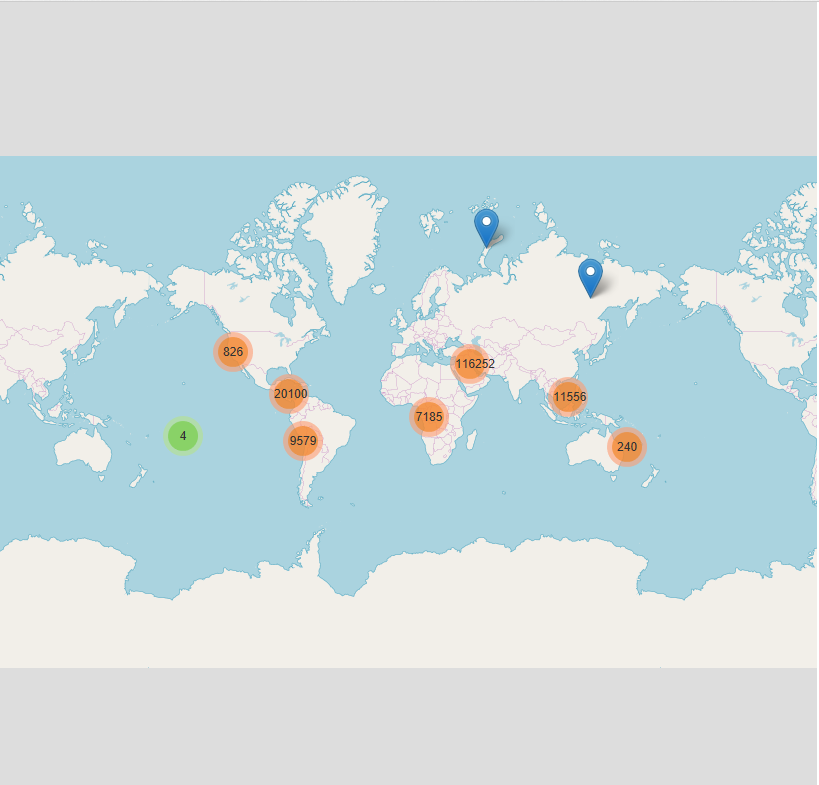
\includegraphics[width=0.9\linewidth]{C:/Users/Tom Kennon/Documents/UCONN/STAT 4185/Project Global Terrorism/Project Progress Report/screenshot1} \end{center}

\begin{center}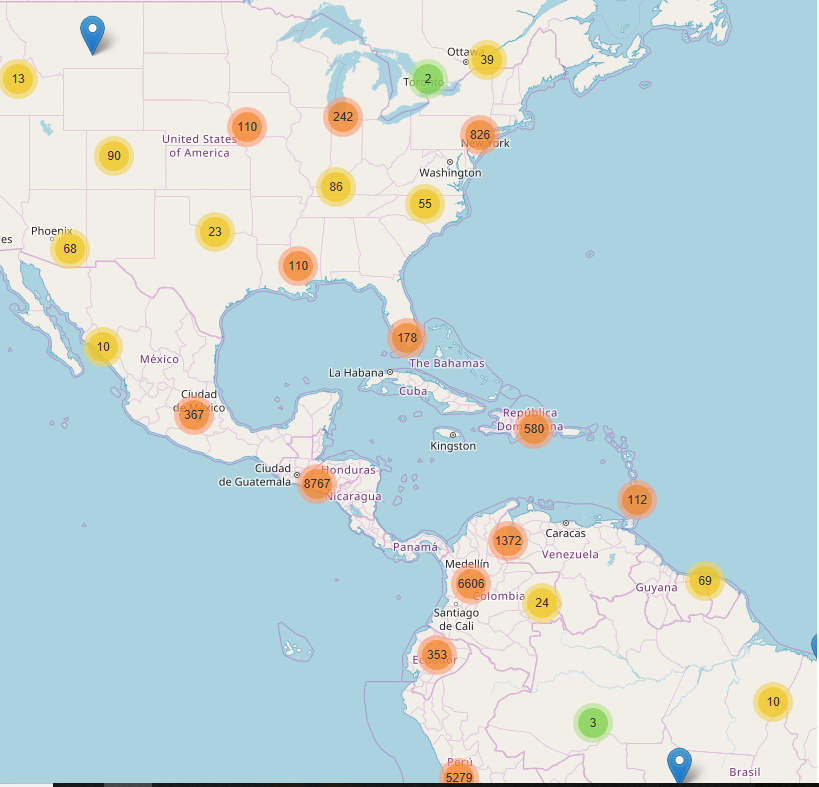
\includegraphics[width=0.9\linewidth]{C:/Users/Tom Kennon/Documents/UCONN/STAT 4185/Project Global Terrorism/Project Progress Report/screenshot2} \end{center}

\begin{center}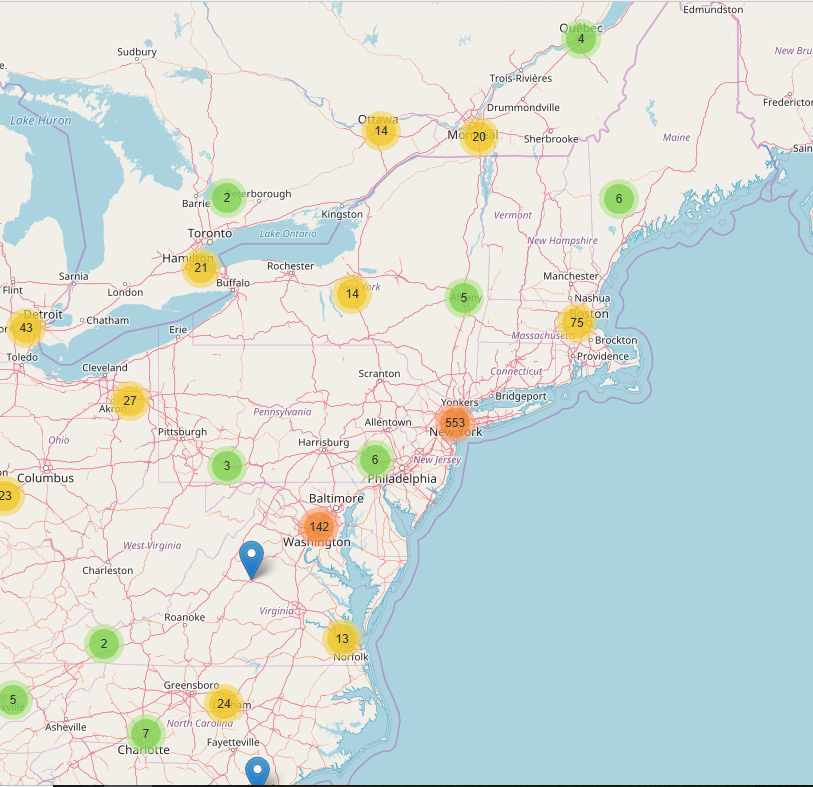
\includegraphics[width=0.9\linewidth]{C:/Users/Tom Kennon/Documents/UCONN/STAT 4185/Project Global Terrorism/Project Progress Report/screenshot3} \end{center}

\begin{center}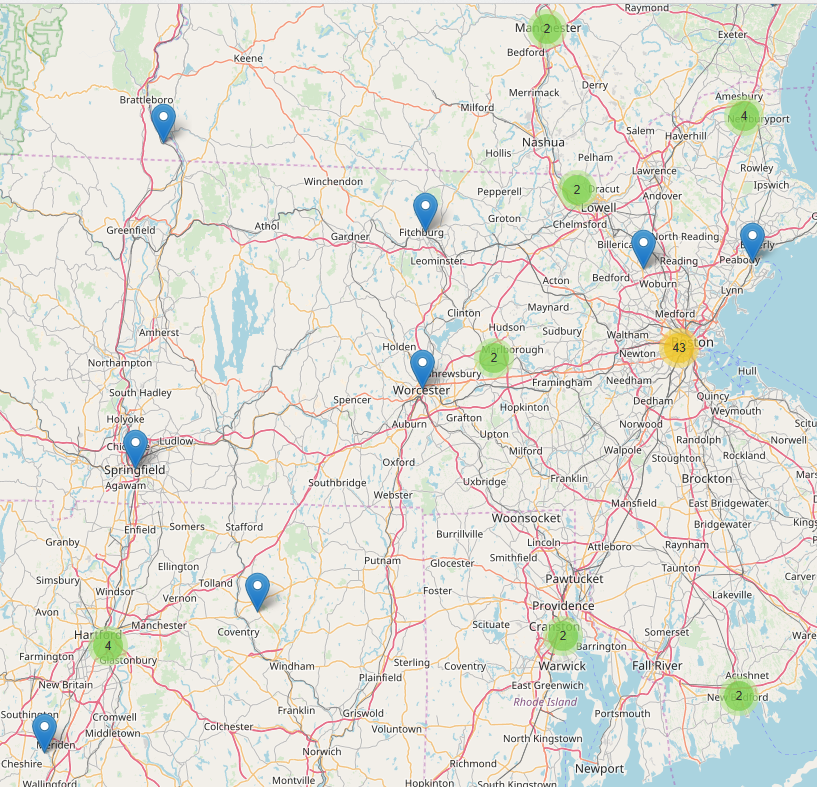
\includegraphics[width=0.9\linewidth]{C:/Users/Tom Kennon/Documents/UCONN/STAT 4185/Project Global Terrorism/Project Progress Report/screenshot4} \end{center}

\begin{center}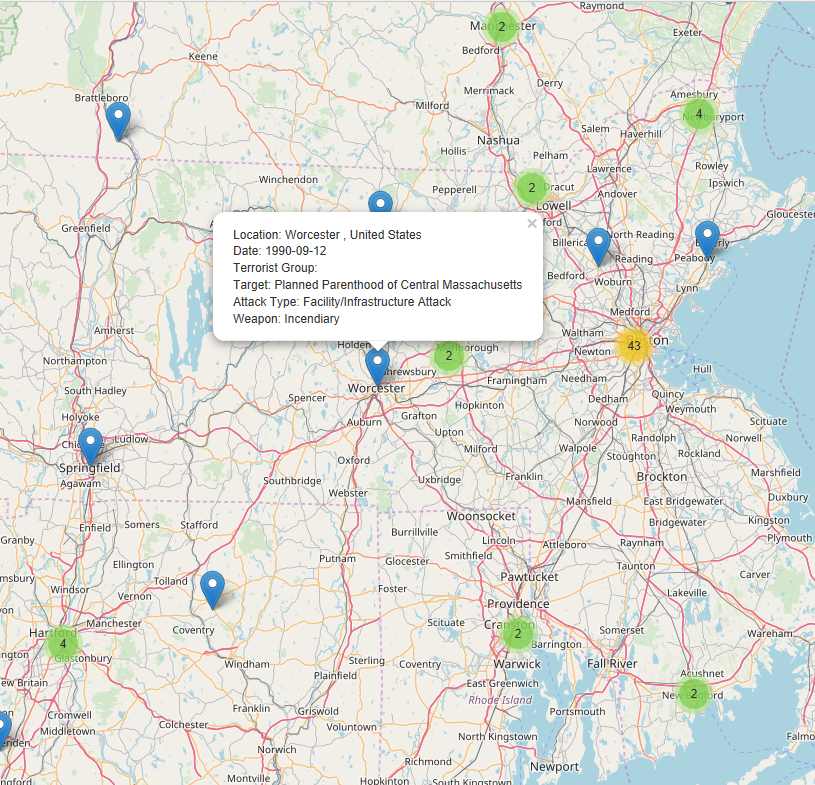
\includegraphics[width=0.9\linewidth]{C:/Users/Tom Kennon/Documents/UCONN/STAT 4185/Project Global Terrorism/Project Progress Report/screenshot5} \end{center}

Above is an interactive geospatial visualization showing all of the
terrorist attacks in this database. Because this is an html document,
you can use the interactive map to find whatever terrorist attacks that
interest you. When a popup is chosen, the location, date, terrorist
group, target name, attack type, and weapon type are displayed. This map
highlights where many terrorist attacks are. The Middle East area has a
lot of attacks. To see a more detailed number for each country or
region, see the following two outputs.

Rank of Number of Attacks for each Country with Descending Order.

\begin{Shaded}
\begin{Highlighting}[]
\NormalTok{## Rank of number of attacks for each country with descending order. }
\NormalTok{gt %>%}
\StringTok{  }\KeywordTok{group_by}\NormalTok{(country_txt) %>%}
\StringTok{  }\KeywordTok{summarise}\NormalTok{( }\DataTypeTok{nr_of_attacks =} \KeywordTok{n}\NormalTok{()) %>%}
\StringTok{  }\KeywordTok{arrange}\NormalTok{(}\KeywordTok{desc}\NormalTok{(nr_of_attacks)) %>%}
\StringTok{  }\KeywordTok{head}\NormalTok{(}\DataTypeTok{n=}\DecValTok{10}\NormalTok{)}
\end{Highlighting}
\end{Shaded}

\begin{verbatim}
## # A tibble: 10 x 2
##    country_txt    nr_of_attacks
##    <fct>                  <int>
##  1 Iraq                   22130
##  2 Pakistan               13634
##  3 Afghanistan            11306
##  4 India                  10978
##  5 Colombia                8163
##  6 Philippines             6212
##  7 Peru                    6088
##  8 El Salvador             5320
##  9 United Kingdom          5098
## 10 Turkey                  4106
\end{verbatim}

As evidenced by the output above, Iraq has the most number of attacks,
followed by Pakistan, Afghanistan, etc. These countries have been known
to have had a lot of terrorist attacks and this is backed in our
findings as well.

Rank of Number of Attacks for each Region with Descending Order.

\begin{Shaded}
\begin{Highlighting}[]
\NormalTok{## Rank by region}
\NormalTok{gt %>%}
\StringTok{  }\KeywordTok{group_by}\NormalTok{(region_txt) %>%}
\StringTok{  }\KeywordTok{summarise}\NormalTok{(}\DataTypeTok{attacks =} \KeywordTok{n}\NormalTok{()) %>%}
\StringTok{  }\KeywordTok{arrange}\NormalTok{(}\KeywordTok{desc}\NormalTok{(attacks)) %>%}
\StringTok{  }\KeywordTok{head}\NormalTok{(}\DataTypeTok{n=}\DecValTok{10}\NormalTok{)}
\end{Highlighting}
\end{Shaded}

\begin{verbatim}
## # A tibble: 10 x 2
##    region_txt                  attacks
##    <fct>                         <int>
##  1 Middle East & North Africa    46511
##  2 South Asia                    41497
##  3 South America                 18762
##  4 Western Europe                16307
##  5 Sub-Saharan Africa            15491
##  6 Southeast Asia                11453
##  7 Central America & Caribbean   10340
##  8 Eastern Europe                 5031
##  9 North America                  3346
## 10 East Asia                       794
\end{verbatim}

As evidenced by the output above, the Middle East and North Africa and
South Asia have the most number of attacks which has been echoed in
world news lately due to shifting political regimes.

Wordcloud of Summaries of Global Terrorist Attacks Since 1970

\begin{Shaded}
\begin{Highlighting}[]
\KeywordTok{library}\NormalTok{(tm)}
\KeywordTok{library}\NormalTok{(SnowballC)}
\KeywordTok{library}\NormalTok{(wordcloud)}

\NormalTok{corpus <-}\StringTok{ }\KeywordTok{Corpus}\NormalTok{(}\KeywordTok{VectorSource}\NormalTok{(gt$summary))}
\NormalTok{corpus <-}\StringTok{ }\KeywordTok{tm_map}\NormalTok{(corpus,removePunctuation)}
\NormalTok{corpus <-}\StringTok{ }\KeywordTok{tm_map}\NormalTok{(corpus,removeWords,}\KeywordTok{c}\NormalTok{(}\StringTok{"the"}\NormalTok{,}\StringTok{"this"}\NormalTok{,}\KeywordTok{stopwords}\NormalTok{(}\StringTok{"english"}\NormalTok{)))}
\NormalTok{corpus <-}\StringTok{ }\KeywordTok{tm_map}\NormalTok{(corpus,stemDocument)}

\KeywordTok{wordcloud}\NormalTok{(corpus,}\DataTypeTok{max.words=}\DecValTok{100}\NormalTok{,}\DataTypeTok{random.order=}\OtherTok{FALSE}\NormalTok{)}
\end{Highlighting}
\end{Shaded}

\begin{center}\includegraphics[width=0.9\linewidth]{FINAL_writeup_files/figure-latex/wordcloud-1} \end{center}

The above plot shows a wordcloud visualization of detailed summaries of
these terrorist attacks. The most frequent word used in the descriptive
summaries for these attacks is ``response'', followed by ``attack'',
``claim'', and ``group''. This is a good way to visualize what is
important to know while investigating terrorist attacks so this aids us
in our analysis.



\begin{Shaded}
\begin{Highlighting}[]
\NormalTok{################}
\NormalTok{### Figure 1 ###}
\NormalTok{################}


\NormalTok{## Bar chart}
\KeywordTok{ggplot}\NormalTok{(gt,}\KeywordTok{aes}\NormalTok{(attacktype1)) +}
\StringTok{  }\KeywordTok{geom_bar}\NormalTok{(}\KeywordTok{aes}\NormalTok{(}\DataTypeTok{fill=}\NormalTok{attacktype1_txt)) +}
\StringTok{  }\KeywordTok{labs}\NormalTok{(}\DataTypeTok{title=}\StringTok{"Attack Types"}\NormalTok{, }\DataTypeTok{y=}\StringTok{"Count"}\NormalTok{, }\DataTypeTok{x=}\StringTok{""}\NormalTok{) +}
\StringTok{  }\KeywordTok{theme}\NormalTok{(}\DataTypeTok{axis.title.x=}\KeywordTok{element_blank}\NormalTok{(),}
        \DataTypeTok{axis.text.x=}\KeywordTok{element_blank}\NormalTok{(),}
        \DataTypeTok{axis.ticks.x=}\KeywordTok{element_blank}\NormalTok{()) +}
\StringTok{  }\KeywordTok{guides}\NormalTok{(}\DataTypeTok{fill=}\KeywordTok{guide_legend}\NormalTok{(}\DataTypeTok{title=}\StringTok{"Attack Type"}\NormalTok{))}
\end{Highlighting}
\end{Shaded}

\begin{figure}

{\centering \includegraphics[width=0.9\linewidth]{FINAL_writeup_files/figure-latex/atype-1} 

}

\caption{Breakdown of Attack Type.}\label{fig:atype}
\end{figure}

In Figure \ref{fig:atype}, we can see that the most popular attack type
in terrorist attacks since 1970 are bombings/explosions followed by
armed assaults and assassinations respectively. But how do these numbers
change over time?



\begin{Shaded}
\begin{Highlighting}[]
\NormalTok{################}
\NormalTok{### Figure 2 ###}
\NormalTok{################}

\NormalTok{cbbPalette <-}\StringTok{ }\KeywordTok{c}\NormalTok{(}\StringTok{"#000000"}\NormalTok{, }\StringTok{"#E69F00"}\NormalTok{, }\StringTok{"#56B4E9"}\NormalTok{, }\StringTok{"#009E73"}\NormalTok{, }\StringTok{"#F0E442"}\NormalTok{, }\StringTok{"#0072B2"}\NormalTok{, }\StringTok{"#D55E00"}\NormalTok{, }\StringTok{"#CC79A7"}\NormalTok{, }\StringTok{"#999999"}\NormalTok{)}

\NormalTok{y<-}\KeywordTok{as.data.frame}\NormalTok{(}\KeywordTok{table}\NormalTok{(gt$iyear, gt$attacktype1_txt))}
\KeywordTok{colnames}\NormalTok{(y) <-}\StringTok{ }\KeywordTok{c}\NormalTok{(}\StringTok{"iyear"}\NormalTok{, }\StringTok{"attacktype1_txt"}\NormalTok{, }\StringTok{"freq"}\NormalTok{)}
\KeywordTok{ggplot}\NormalTok{(}\DataTypeTok{data=}\NormalTok{y) +}
\StringTok{  }\KeywordTok{geom_point}\NormalTok{(}\DataTypeTok{mapping =} \KeywordTok{aes}\NormalTok{(}\DataTypeTok{x=}\NormalTok{iyear, }\DataTypeTok{y=}\NormalTok{freq, }\DataTypeTok{color=}\NormalTok{attacktype1_txt))+}
\StringTok{  }\KeywordTok{scale_color_manual}\NormalTok{(}\DataTypeTok{values=}\NormalTok{cbbPalette) +}
\StringTok{  }\KeywordTok{scale_x_discrete}\NormalTok{(}\DataTypeTok{breaks=}\KeywordTok{c}\NormalTok{(}\DecValTok{1970}\NormalTok{,}\DecValTok{1980}\NormalTok{,}\DecValTok{1990}\NormalTok{,}\DecValTok{2000}\NormalTok{,}\DecValTok{2010}\NormalTok{))}
\end{Highlighting}
\end{Shaded}

\begin{figure}

{\centering \includegraphics[width=0.9\linewidth]{FINAL_writeup_files/figure-latex/ayear1-1} 

}

\caption{Scatterplot: Trends in Attack Types Since 1970.}\label{fig:ayear1}
\end{figure}



\begin{Shaded}
\begin{Highlighting}[]
\NormalTok{################}
\NormalTok{### Figure 3 ###}
\NormalTok{################}

\KeywordTok{ggplot}\NormalTok{(}\DataTypeTok{data=}\NormalTok{gt) +}
\StringTok{  }\KeywordTok{geom_count}\NormalTok{(}\DataTypeTok{mapping =} \KeywordTok{aes}\NormalTok{(}\DataTypeTok{x=}\NormalTok{iyear, }\DataTypeTok{y=}\NormalTok{attacktype1_txt)) +}
\StringTok{  }\KeywordTok{scale_x_discrete}\NormalTok{(}\DataTypeTok{breaks=}\KeywordTok{c}\NormalTok{(}\DecValTok{1970}\NormalTok{,}\DecValTok{1980}\NormalTok{,}\DecValTok{1990}\NormalTok{,}\DecValTok{2000}\NormalTok{,}\DecValTok{2010}\NormalTok{))}
\end{Highlighting}
\end{Shaded}

\begin{figure}

{\centering \includegraphics[width=0.9\linewidth]{FINAL_writeup_files/figure-latex/ayear2-1} 

}

\caption{Bubblechart: Trends in Attack Types Since 1970.}\label{fig:ayear2}
\end{figure}

In Figure \ref{fig:ayear2} and Figure \ref{fig:ayear1}, we have created
2 different graphs that illustrate trends in attack types since 1970. In
it we can clearly see there has been a large spike in bombings in recent
years, as well as a mild spike in armed assault. While most other
methods have seen an increase in recent years, these two are by far the
greatest increase. This may imply that these are simply the preferred
methods by groups that started up since the late 1990's/early 2000's. It
could also mean that terrorist groups have just experienced more success
with these methods, and thus have been utilizing them more. We have the
necessary data to test both of these possibilities. Another interesting
variable to look into is the terrorist group.



\begin{Shaded}
\begin{Highlighting}[]
\NormalTok{################}
\NormalTok{### Figure 4 ###}
\NormalTok{################}


\NormalTok{## Identify major terrorist organizations}
\NormalTok{terr.groups <-}\StringTok{ }\NormalTok{gt %>%}\StringTok{ }
\StringTok{  }\KeywordTok{select}\NormalTok{(gname, success) %>%}\StringTok{ }
\StringTok{  }\KeywordTok{filter}\NormalTok{(!gname %in%}\StringTok{ "Unknown"}\NormalTok{) %>%}\StringTok{ }
\StringTok{  }\KeywordTok{group_by}\NormalTok{(gname) %>%}\StringTok{ }
\StringTok{  }\KeywordTok{summarise}\NormalTok{(}\DataTypeTok{n.success=}\KeywordTok{sum}\NormalTok{(success)) %>%}\StringTok{ }
\StringTok{  }\KeywordTok{arrange}\NormalTok{(}\KeywordTok{desc}\NormalTok{(n.success)) %>%}\StringTok{ }
\StringTok{  }\KeywordTok{filter}\NormalTok{(n.success >=}\StringTok{ }\DecValTok{1500}\NormalTok{) }\CommentTok{#this will filter out any terrorist groups with less than 1500 successful attacks}

\NormalTok{terr.groups$n.success <-}\StringTok{ }\KeywordTok{as.numeric}\NormalTok{(terr.groups$n.success)}

\NormalTok{## Bar chart}
\KeywordTok{ggplot}\NormalTok{(terr.groups, }\KeywordTok{aes}\NormalTok{(gname, n.success)) +}
\StringTok{  }\KeywordTok{geom_bar}\NormalTok{(}\DataTypeTok{stat=}\StringTok{"identity"}\NormalTok{,}\KeywordTok{aes}\NormalTok{(}\DataTypeTok{fill=}\NormalTok{gname)) +}
\StringTok{  }\KeywordTok{labs}\NormalTok{(}\DataTypeTok{title=}\StringTok{"Successful Attacks by Group Name"}\NormalTok{, }\DataTypeTok{y=}\StringTok{"Successes"}\NormalTok{, }\DataTypeTok{x=}\StringTok{""}\NormalTok{) +}
\StringTok{  }\KeywordTok{theme}\NormalTok{(}\DataTypeTok{axis.title.x=}\KeywordTok{element_blank}\NormalTok{(),}
        \DataTypeTok{axis.text.x=}\KeywordTok{element_blank}\NormalTok{(),}
        \DataTypeTok{axis.ticks.x=}\KeywordTok{element_blank}\NormalTok{()) +}
\StringTok{  }\KeywordTok{guides}\NormalTok{(}\DataTypeTok{fill=}\KeywordTok{guide_legend}\NormalTok{(}\DataTypeTok{title=}\StringTok{"Group Name"}\NormalTok{))}
\end{Highlighting}
\end{Shaded}

\begin{figure}

{\centering \includegraphics[width=0.9\linewidth]{FINAL_writeup_files/figure-latex/group-1} 

}

\caption{Successful Terrorist Groups}\label{fig:group}
\end{figure}

In Figure \ref{fig:group} we can see the which terrorist groups have the
most successful attacks. The Taliban has the most successful attacks at
approximately 6000 and the Shining Path (SL) and Islamic State of Iraq
and the Levant (ISIL) have the second and third most respectively.



\begin{Shaded}
\begin{Highlighting}[]
\NormalTok{################}
\NormalTok{### Figure 5 ###}
\NormalTok{################}

\NormalTok{## Over time}
\NormalTok{gname.line <-}\StringTok{ }\NormalTok{gt %>%}\StringTok{ }
\StringTok{  }\KeywordTok{select}\NormalTok{(gname,iyear,success) %>%}\StringTok{ }
\StringTok{  }\KeywordTok{group_by}\NormalTok{(gname,iyear) %>%}\StringTok{ }
\StringTok{  }\KeywordTok{summarise}\NormalTok{(}\DataTypeTok{n.success =} \KeywordTok{sum}\NormalTok{(success)) %>%}\StringTok{ }
\StringTok{  }\KeywordTok{filter}\NormalTok{(gname %in%}\StringTok{ }\KeywordTok{c}\NormalTok{(}\StringTok{"Al-Shabaab"}\NormalTok{,}\StringTok{"Basque Fatherland and Freedom (ETA)"}\NormalTok{, }\StringTok{"Boko Haram"}\NormalTok{, }\StringTok{"Communist Party of India - Maoist (CPI-Maoist)"}\NormalTok{, }\StringTok{"Farabundo Marti National Liberation Front (FMLN)"}\NormalTok{, }\StringTok{"Irish Republican Army (IRA)"}\NormalTok{, }\StringTok{"Islamic State of Iraq and the Levant (ISIL)"}\NormalTok{, }\StringTok{"Kurdistan Workers' Party (PKK)"}\NormalTok{, }\StringTok{"Liberation Tigers of Tamil Eelam (LTTE)"}\NormalTok{, }\StringTok{"New People's Army (NPA)"}\NormalTok{, }\StringTok{"Revolutionary Armed Forces of Columbia (FARC)"}\NormalTok{, }\StringTok{"Shining Path (SL)"}\NormalTok{, }\StringTok{"Taliban"}\NormalTok{))}

\NormalTok{gname.line$iyear <-}\StringTok{ }\KeywordTok{as.numeric}\NormalTok{(gname.line$iyear)}

\KeywordTok{ggplot}\NormalTok{(gname.line,}\KeywordTok{aes}\NormalTok{(iyear, n.success)) +}
\StringTok{  }\KeywordTok{geom_line}\NormalTok{(}\KeywordTok{aes}\NormalTok{(}\DataTypeTok{color=}\NormalTok{gname)) +}
\StringTok{  }\KeywordTok{labs}\NormalTok{(}\DataTypeTok{title=}\StringTok{"Terrorist Group Activity Since 1970"}\NormalTok{, }\DataTypeTok{y=}\StringTok{"Successes"}\NormalTok{, }\DataTypeTok{x=}\StringTok{""}\NormalTok{) +}
\StringTok{  }\KeywordTok{guides}\NormalTok{(}\DataTypeTok{fill=}\KeywordTok{guide_legend}\NormalTok{(}\DataTypeTok{title=}\StringTok{"Group Name"}\NormalTok{)) +}
\StringTok{  }\KeywordTok{scale_x_discrete}\NormalTok{(}\DataTypeTok{breaks=}\KeywordTok{c}\NormalTok{(}\DecValTok{1970}\NormalTok{,}\DecValTok{1980}\NormalTok{,}\DecValTok{1990}\NormalTok{,}\DecValTok{2000}\NormalTok{,}\DecValTok{2010}\NormalTok{))}
\end{Highlighting}
\end{Shaded}

\begin{figure}

{\centering \includegraphics[width=0.9\linewidth]{FINAL_writeup_files/figure-latex/group2-1} 

}

\caption{Successful Terrorist Groups Over Time}\label{fig:group2}
\end{figure}

In Figure \ref{fig:group2} we can see the which terrorist groups have
the most successful attacks over time. This is a useful insight that
adds to Figure \ref{fig:group} because now it is evident which groups
have had an influx in attacks as of late compared to groups that have
died out. Al-Shabaab has only had attacks since 2007, while the Irish
Republican Army used to have a lot of terrorist attacks but not as many
as of recently. The Islamic State of Iraq and the Levant (ISIL)'s
terrorist attacks have only had attacks as of 2013 yet have the third
most successful terrorist attacks in data back to 1970 so they are a
scary threat.



\begin{Shaded}
\begin{Highlighting}[]
\NormalTok{################}
\NormalTok{### Figure 6 ###}
\NormalTok{################}


\NormalTok{## number of terrorist attacks over time}
\KeywordTok{ggplot}\NormalTok{(gt, }\KeywordTok{aes}\NormalTok{(}\DataTypeTok{x=}\NormalTok{iyear)) +}
\StringTok{  }\KeywordTok{geom_histogram}\NormalTok{(}\DataTypeTok{stat=}\StringTok{'count'}\NormalTok{) +}
\StringTok{  }\KeywordTok{labs}\NormalTok{(}\DataTypeTok{title=}\StringTok{'Terrorism attacks over time'}\NormalTok{) +}
\StringTok{  }\KeywordTok{scale_x_discrete}\NormalTok{(}\DataTypeTok{breaks=}\KeywordTok{c}\NormalTok{(}\DecValTok{1970}\NormalTok{,}\DecValTok{1980}\NormalTok{,}\DecValTok{1990}\NormalTok{,}\DecValTok{2000}\NormalTok{,}\DecValTok{2010}\NormalTok{))}
\end{Highlighting}
\end{Shaded}

\begin{figure}

{\centering \includegraphics[width=0.9\linewidth]{FINAL_writeup_files/figure-latex/attacksovertime-1} 

}

\caption{Plot of Terrorist Attacks Over Time.}\label{fig:attacksovertime}
\end{figure}




\begin{Shaded}
\begin{Highlighting}[]
\NormalTok{################}
\NormalTok{### Figure 7 ###}
\NormalTok{################}

\NormalTok{## plot terrorism growth versus population growth}
\NormalTok{p1 <-}\StringTok{ }\KeywordTok{ggplot}\NormalTok{(}\DataTypeTok{data=}\NormalTok{popworld2, }\KeywordTok{aes}\NormalTok{(}\DataTypeTok{x=}\NormalTok{year)) +}
\StringTok{  }\KeywordTok{geom_histogram}\NormalTok{(}\KeywordTok{aes}\NormalTok{(}\DataTypeTok{col=}\StringTok{'Attack Count'}\NormalTok{),}\DataTypeTok{bins=}\DecValTok{45}\NormalTok{) +}\StringTok{ }
\StringTok{  }\KeywordTok{scale_x_continuous}\NormalTok{(}\DataTypeTok{breaks=}\KeywordTok{seq}\NormalTok{(}\DecValTok{1970}\NormalTok{, }\DecValTok{2016}\NormalTok{, }\DecValTok{10}\NormalTok{))}

\NormalTok{p1+}\StringTok{ }\KeywordTok{geom_line}\NormalTok{(}\KeywordTok{aes}\NormalTok{(}\DataTypeTok{y=}\NormalTok{population/}\DecValTok{500000}\NormalTok{, }\DataTypeTok{col=}\StringTok{'Population'}\NormalTok{)) +}\StringTok{ }
\StringTok{    }\KeywordTok{scale_y_continuous}\NormalTok{(}\DataTypeTok{sec.axis =} \KeywordTok{sec_axis}\NormalTok{(~}\StringTok{ }\NormalTok{. *}\StringTok{ }\DecValTok{500000}\NormalTok{, }\DataTypeTok{name =} \StringTok{"Population Size"}\NormalTok{))+}
\StringTok{    }\KeywordTok{labs}\NormalTok{(}\DataTypeTok{y =} \StringTok{"Attack Count"}\NormalTok{, }\DataTypeTok{x =} \StringTok{"Year"}\NormalTok{, }\DataTypeTok{colour =} \StringTok{"Blue"}\NormalTok{) +}
\StringTok{    }\KeywordTok{labs}\NormalTok{(}\DataTypeTok{title=}\StringTok{"Terrorism growth vs Population growth"}\NormalTok{)}
\end{Highlighting}
\end{Shaded}

\begin{figure}

{\centering \includegraphics[width=0.9\linewidth]{FINAL_writeup_files/figure-latex/terrvspop-1} 

}

\caption{Plot of Terrorism Growth vs.~World Population Growth
Over Time}\label{fig:terrvspop}
\end{figure}

As evidenced by Figure \ref{fig:attacksovertime}, there is an increase
in terrorist attacks as the year increases. However, there is also an
increase in the general world population as we know from our merge with
the world population dataset. One can see from viewing Figure
\ref{fig:terrvspop}, that there is still a rapid increase in terrorist
attacks even accounting for world population size aka there is still an
increasing amount of terrorist attacks per capita as the years increase
which relates to one of our main questions.



\begin{Shaded}
\begin{Highlighting}[]
\NormalTok{################}
\NormalTok{### Figure 8 ###}
\NormalTok{################}

\NormalTok{## Worldwide killings grouped by year}
\NormalTok{datakill <-}\StringTok{ }\NormalTok{gt %>%}\StringTok{ }\KeywordTok{filter}\NormalTok{(nkill>}\DecValTok{0}\NormalTok{)}
\NormalTok{data_1<-datakill %>%}\StringTok{ }\KeywordTok{group_by}\NormalTok{(iyear) %>%}\StringTok{ }\KeywordTok{summarise}\NormalTok{(}\DataTypeTok{n=}\KeywordTok{sum}\NormalTok{(nkill))}
\KeywordTok{colnames}\NormalTok{(data_1)<-}\KeywordTok{c}\NormalTok{(}\StringTok{"Year"}\NormalTok{,}\StringTok{"Killed"}\NormalTok{)}
\NormalTok{data_1$Year <-}\StringTok{ }\KeywordTok{as.numeric}\NormalTok{(data_1$Year)}
\NormalTok{data_1$Killed <-}\StringTok{ }\KeywordTok{as.numeric}\NormalTok{(data_1$Killed)}
\NormalTok{p2<-}\KeywordTok{ggplot}\NormalTok{(data_1,}\KeywordTok{aes}\NormalTok{(}\DataTypeTok{x=}\NormalTok{Year,}\DataTypeTok{y=}\NormalTok{Killed))+}
\StringTok{  }\KeywordTok{geom_line}\NormalTok{()+}\KeywordTok{theme_bw}\NormalTok{()}
\NormalTok{p2}
\end{Highlighting}
\end{Shaded}

\begin{figure}

{\centering \includegraphics[width=0.9\linewidth]{FINAL_writeup_files/figure-latex/yearkillings-1} 

}

\caption{Worldwide Killings Grouped by Year.}\label{fig:yearkillings}
\end{figure}

As evidenced by Figure \ref{fig:yearkillings}, there is an increasing
trend of number of people killed after 2000 and a very high increasing
trend after 2010. This relates to one of main questions if there is an
increase in terrorist attacks as of recently indicating that there is
not just a recency bias! More people are being killed in terrorist
attacks as the years go on.

\section{Predictive Analytics}\label{predictive-analytics}

\subsection{\texorpdfstring{Predicting ``ISIL'' Terrorist
Group}{Predicting ISIL Terrorist Group}}\label{predicting-isil-terrorist-group}

\subsubsection{Naive Bayes}\label{naive-bayes}

Here we lay out our methodology for the Naive Bayes Model.

\begin{verbatim}
## # A tibble: 170,350 x 135
##         eventid iyear imonth  iday approxdate extended resolution country
##           <dbl> <int>  <int> <int> <fct>         <int> <fct>        <int>
##  1 197000000001  1970      7     2 ""                0 ""              58
##  2 197000000002  1970      0     0 ""                0 ""             130
##  3 197001000001  1970      1     0 ""                0 ""             160
##  4 197001000002  1970      1     0 ""                0 ""              78
##  5 197001000003  1970      1     0 ""                0 ""             101
##  6 197001010002  1970      1     1 ""                0 ""             217
##  7 197001020001  1970      1     2 ""                0 ""             218
##  8 197001020002  1970      1     2 ""                0 ""             217
##  9 197001020003  1970      1     2 ""                0 ""             217
## 10 197001030001  1970      1     3 ""                0 ""             217
## # ... with 170,340 more rows, and 127 more variables: country_txt <fct>,
## #   region <int>, region_txt <fct>, provstate <fct>, city <fct>,
## #   latitude <dbl>, longitude <dbl>, specificity <int>, vicinity <int>,
## #   location <fct>, summary <fct>, crit1 <int>, crit2 <int>, crit3 <int>,
## #   doubtterr <int>, alternative <int>, alternative_txt <fct>,
## #   multiple <int>, success <int>, suicide <int>, attacktype1 <int>,
## #   attacktype1_txt <fct>, attacktype2 <int>, attacktype2_txt <fct>,
## #   attacktype3 <int>, attacktype3_txt <fct>, targtype1 <int>,
## #   targtype1_txt <fct>, targsubtype1 <int>, targsubtype1_txt <fct>,
## #   corp1 <fct>, target1 <fct>, natlty1 <int>, natlty1_txt <fct>,
## #   targtype2 <int>, targtype2_txt <fct>, targsubtype2 <int>,
## #   targsubtype2_txt <fct>, corp2 <fct>, target2 <fct>, natlty2 <int>,
## #   natlty2_txt <fct>, targtype3 <int>, targtype3_txt <fct>,
## #   targsubtype3 <int>, targsubtype3_txt <fct>, corp3 <fct>,
## #   target3 <fct>, natlty3 <int>, natlty3_txt <fct>, gname <fct>,
## #   gsubname <fct>, gname2 <fct>, gsubname2 <fct>, gname3 <fct>,
## #   gsubname3 <fct>, motive <fct>, guncertain1 <int>, guncertain2 <int>,
## #   guncertain3 <int>, individual <int>, nperps <int>, nperpcap <dbl>,
## #   claimed <int>, claimmode <int>, claimmode_txt <fct>, claim2 <int>,
## #   claimmode2 <int>, claimmode2_txt <fct>, claim3 <int>,
## #   claimmode3 <int>, claimmode3_txt <fct>, compclaim <int>,
## #   weaptype1 <int>, weaptype1_txt <fct>, weapsubtype1 <int>,
## #   weapsubtype1_txt <fct>, weaptype2 <int>, weaptype2_txt <fct>,
## #   weapsubtype2 <int>, weapsubtype2_txt <fct>, weaptype3 <int>,
## #   weaptype3_txt <fct>, weapsubtype3 <int>, weapsubtype3_txt <fct>,
## #   weaptype4 <int>, weaptype4_txt <fct>, weapsubtype4 <int>,
## #   weapsubtype4_txt <fct>, weapdetail <fct>, nkill <int>, nkillus <int>,
## #   nkillter <int>, nwound <int>, nwoundus <int>, nwoundte <int>,
## #   property <int>, propextent <int>, propextent_txt <fct>,
## #   propvalue <dbl>, ...
\end{verbatim}

\begin{Shaded}
\begin{Highlighting}[]
\KeywordTok{tally}\NormalTok{(~Isil, }\DataTypeTok{data=}\NormalTok{train, }\DataTypeTok{format=}\StringTok{"percent"}\NormalTok{)}
\end{Highlighting}
\end{Shaded}

\begin{verbatim}
## Isil
##         0         1 
## 92.501694  7.498306
\end{verbatim}

\begin{Shaded}
\begin{Highlighting}[]
\NormalTok{## Creating a null model, shows 7.5 % of attacks are known to be carried out by ISIL}

\NormalTok{form<-}\KeywordTok{as.formula}\NormalTok{(}\StringTok{"Isil~iyear+region_txt+attacktype1_txt+targtype1_txt+weaptype1_txt"}\NormalTok{)}
\NormalTok{## Creating a model using the country, attack type, target type,}
\NormalTok{##  and weapon type as predictors}
\end{Highlighting}
\end{Shaded}

Our null model shows that 7.5\% of terrorist attacks are to be carried
out by ISIL, so this is the model to beat. We also write our formula to
use for the Naive Bayes modelling. We use ISIL (coded 0 for non-ISIL
terrorist group and 1 for ISIL terrorist group) as the dependent
variable. The predictors we threw into the model include year the attack
happened, region of the world where the attack occurred, the attack
type, the target type, and the weapon type.

Here is our Naive Bayes model fitting and our corresponding predictions
for the training and testing set.

\begin{Shaded}
\begin{Highlighting}[]
\NormalTok{mod_NB_train<-}\KeywordTok{naiveBayes}\NormalTok{(form, }\DataTypeTok{data=}\NormalTok{train)}
\NormalTok{## Naive Bayes model for Training Data}

\NormalTok{pred_NB_train<-}\KeywordTok{predict}\NormalTok{(mod_NB_train, }\DataTypeTok{newdata=}\NormalTok{train)}
\NormalTok{## Prediction using the Naive Bayes model for Training Data}

\NormalTok{mod_NB_test<-}\KeywordTok{naiveBayes}\NormalTok{(form, }\DataTypeTok{data=}\NormalTok{test)}
\NormalTok{## Naive Bayes model for Testing Data}

\NormalTok{pred_NB_test<-}\KeywordTok{predict}\NormalTok{(mod_NB_test, }\DataTypeTok{newdata=}\NormalTok{test)}
\NormalTok{## Prediction using the Naive Bayes model for Testing Data}
\end{Highlighting}
\end{Shaded}

\begin{Shaded}
\begin{Highlighting}[]
\NormalTok{confusion_train <-}\StringTok{ }\KeywordTok{table}\NormalTok{(pred_NB_train, train$success)}
\NormalTok{confusion_train}
\end{Highlighting}
\end{Shaded}

\begin{verbatim}
##              
## pred_NB_train     0     1
##             0  6372 37973
##             1   253  1159
\end{verbatim}

\begin{Shaded}
\begin{Highlighting}[]
\NormalTok{## Confusion Matrix for Training Set}

\NormalTok{Accuracy_train <-}\KeywordTok{sum}\NormalTok{(}\KeywordTok{diag}\NormalTok{(confusion_train))   /}\StringTok{ }\KeywordTok{nrow}\NormalTok{(train)}
\NormalTok{Accuracy_train}
\end{Highlighting}
\end{Shaded}

\begin{verbatim}
## [1] 0.1645868
\end{verbatim}

\begin{Shaded}
\begin{Highlighting}[]
\NormalTok{## Our training set appears to have been predicted with about 16.46 percent accuracy}


\NormalTok{confusion_test <-}\StringTok{ }\KeywordTok{table}\NormalTok{(pred_NB_test, test$success)}
\NormalTok{confusion_test}
\end{Highlighting}
\end{Shaded}

\begin{verbatim}
##             
## pred_NB_test    0    1
##            0 1578 9624
##            1   61  176
\end{verbatim}

\begin{Shaded}
\begin{Highlighting}[]
\NormalTok{## Confusion Matrix for Test set}


\NormalTok{Accuracy_test <-}\KeywordTok{sum}\NormalTok{(}\KeywordTok{diag}\NormalTok{(confusion_test))   /}\StringTok{ }\KeywordTok{nrow}\NormalTok{(test)}
\NormalTok{Accuracy_test}
\end{Highlighting}
\end{Shaded}

\begin{verbatim}
## [1] 0.1533351
\end{verbatim}

\begin{Shaded}
\begin{Highlighting}[]
\NormalTok{## The test set was predicted with about 15.33 percent accuracy}
\NormalTok{## Overall, the model does not appear to be overfitted, and this is an improvement from the null model}
\end{Highlighting}
\end{Shaded}

Here we are trying to predict whether a terrorist attack was carried out
by ISIL, utilizing weapon type, target type, attack type, and country as
predictors. To do this effectively, we limit the data to only the years
2013-2016, as these are the years when ISIL became more active in their
attacks (as seen in our descriptive analysis seen in Figure
\ref{fig:group2}). Our null model showed that if we assume all attacks
are committed by ISIL, we are only right about 7.5 percent of the time.
However, we were able to correctly determine if an attack was carried
out by ISIL with 17.67 percent accuracy in our training set, and with
about 17.21 percent accuracy in our testing set. These accuracies are a
decent improvement over the null model, and are close enough that we are
not concerned with overfitting. In this example we have laid out the
general framework for a Naive Bayes classification so in our future
analysis discussing Naive Bayes we will only provide and interpret the
output rather than show all of our code.

\subsection{Predicting Mass Terrorist Attacks (\textgreater{}3
Deaths)}\label{predicting-mass-terrorist-attacks-3-deaths}

In this section, we show which predictors could lead to mass terrorist
attacks. We want to investigate mass terrorism in our dataset. We define
a ``mass terrorist attack'' as an attack that killed more than three
people (3 kills is the 85th percentile of the \emph{nkill} variable in
our dataset). We drop any missing values in the \emph{nkill} variable.

\begin{verbatim}
##   0%  25%  50%  75%  85%  90% 100% 
##    0    0    0    2    3    5 1500
\end{verbatim}

\subsubsection{Decision Tree}\label{decision-tree}

\begin{Shaded}
\begin{Highlighting}[]
\KeywordTok{tally}\NormalTok{(~massTerr, }\DataTypeTok{data=}\NormalTok{train,}\DataTypeTok{format=}\StringTok{"percent"}\NormalTok{) }\CommentTok{#null model has 85.62% accuracy}
\end{Highlighting}
\end{Shaded}

\begin{verbatim}
## massTerr
##        0        1 
## 85.61937 14.38063
\end{verbatim}

\begin{Shaded}
\begin{Highlighting}[]
\NormalTok{## Null model}

   
\NormalTok{mod_tree <-}\StringTok{ }\KeywordTok{rpart}\NormalTok{(massTerr ~}\StringTok{ }\NormalTok{., }\DataTypeTok{data =} \NormalTok{train, }\DataTypeTok{method =} \StringTok{"class"}\NormalTok{,}\DataTypeTok{control =} \KeywordTok{rpart.control}\NormalTok{(}\DataTypeTok{cp =} \FloatTok{0.01}\NormalTok{))}
\CommentTok{#mod_tree}
\NormalTok{## Builds Decision Tree }
\end{Highlighting}
\end{Shaded}



\begin{Shaded}
\begin{Highlighting}[]
\KeywordTok{rpart.plot}\NormalTok{(mod_tree)}
\end{Highlighting}
\end{Shaded}

\begin{figure}

{\centering \includegraphics[width=0.9\linewidth]{FINAL_writeup_files/figure-latex/masstreeplot-1} 

}

\caption{Worldwide Killings Grouped by Year.}\label{fig:masstreeplot}
\end{figure}

\begin{Shaded}
\begin{Highlighting}[]
\NormalTok{## Plots Decision Tree  }
\end{Highlighting}
\end{Shaded}

Our null model shows that 85.62\% of terrorist attacks have 3 or fewer
kills. We also build our decision tree here. We use massTerr (coded 0
for 3 or fewer kills in the terrorist attack and 1 for greater than 3
kills in the terrorist attack) as the dependent variable. The predictors
we threw into the model include the attack type, the year the attack
happened, the target type, the weapon type, extended, if there was a
suicide attempt, and region of the world where the attack occurred.

Based on the plot of this decision tree in Figure
\ref{fig:masstreeplot}, the most important factor used in predicting a
``mass terrorist attack'' was whether or not it was a suicide attack. If
the attack was not a suicide attack (representing about 96\% of the
data), the model decides that the attack was not a mass terrorist
attack. If the attack \emph{was} a suicide (representing about 4\% of
the data), the model then looks to the ``target type'' variable to
determine whether the attack killed more than three people. If the
suicide attack was directed toward some maritime, telecommunication, or
some unknown target, the model decides that the attack was not a mass
terrorist attacks. If the suicide attack was not directed at one of the
aforementioned targets, the model decides that the attack was a mass
terrorist attack.

\begin{Shaded}
\begin{Highlighting}[]
\NormalTok{train.dt <-}\StringTok{ }\NormalTok{train %>%}
\StringTok{  }\KeywordTok{mutate}\NormalTok{(}\DataTypeTok{massTerr_dtree   =} \KeywordTok{predict}\NormalTok{(mod_tree,}\DataTypeTok{type=}\StringTok{"class"}\NormalTok{,}\DataTypeTok{data=}\NormalTok{train))}
\NormalTok{confusion.mass.terr <-}\StringTok{ }\KeywordTok{tally}\NormalTok{(massTerr_dtree   ~}\StringTok{ }\NormalTok{massTerr,}\DataTypeTok{data=}\NormalTok{train.dt,}\DataTypeTok{format=}\StringTok{"count"}\NormalTok{)}
\NormalTok{confusion.mass.terr}
\end{Highlighting}
\end{Shaded}

\begin{verbatim}
##               massTerr
## massTerr_dtree      0      1
##              0 108416  15824
##              1   1634   2660
\end{verbatim}

\begin{Shaded}
\begin{Highlighting}[]
\NormalTok{## Confusion Matrix Training}



\NormalTok{dtAcc.mt <-}\StringTok{ }\KeywordTok{sum}\NormalTok{(}\KeywordTok{diag}\NormalTok{(confusion.mass.terr))  /}\StringTok{ }\KeywordTok{nrow}\NormalTok{(train)}
\NormalTok{dtAcc.mt}
\end{Highlighting}
\end{Shaded}

\begin{verbatim}
## [1] 0.864176
\end{verbatim}

\begin{Shaded}
\begin{Highlighting}[]
\NormalTok{## Accuracy for Training Data}


\NormalTok{test.dt <-}\StringTok{ }\NormalTok{test %>%}
\StringTok{  }\KeywordTok{mutate}\NormalTok{(}\DataTypeTok{massTerr_dtree   =} \KeywordTok{predict}\NormalTok{(mod_tree, }\DataTypeTok{newdata=}\NormalTok{test, }\DataTypeTok{type=}\StringTok{"class"}\NormalTok{))}
\NormalTok{confusion.mass.terr_test <-}\StringTok{ }\KeywordTok{tally}\NormalTok{(massTerr_dtree   ~}\StringTok{ }\NormalTok{massTerr, }\DataTypeTok{data =} \NormalTok{test.dt, }\DataTypeTok{format =} \StringTok{"count"}\NormalTok{)}
\NormalTok{confusion.mass.terr_test}
\end{Highlighting}
\end{Shaded}

\begin{verbatim}
##               massTerr
## massTerr_dtree     0     1
##              0 27132  3924
##              1   416   662
\end{verbatim}

\begin{Shaded}
\begin{Highlighting}[]
\NormalTok{## Confusion Matrix Testing}


\NormalTok{dtAcc.mt_test <-}\StringTok{ }\KeywordTok{sum}\NormalTok{(}\KeywordTok{diag}\NormalTok{(confusion.mass.terr_test))  /}\StringTok{ }\KeywordTok{nrow}\NormalTok{(test)}
\NormalTok{dtAcc.mt_test}
\end{Highlighting}
\end{Shaded}

\begin{verbatim}
## [1] 0.8649406
\end{verbatim}

\begin{Shaded}
\begin{Highlighting}[]
\NormalTok{## Accuracy for Testing Data}


\NormalTok{DT.mt <-}\StringTok{ }\KeywordTok{c}\NormalTok{(dtAcc.mt,dtAcc.mt_test)}
\NormalTok{dtAcc.mt ## Accuracy of Training}
\end{Highlighting}
\end{Shaded}

\begin{verbatim}
## [1] 0.864176
\end{verbatim}

\begin{Shaded}
\begin{Highlighting}[]
\NormalTok{dtAcc.mt_test ## Accuracy of Testing}
\end{Highlighting}
\end{Shaded}

\begin{verbatim}
## [1] 0.8649406
\end{verbatim}

Our null model shows that 85.62\% of terrorist attacks have 3 or fewer
kills. However, we were able to correctly determine if an attack was a
mass terrorist attack with 86.42\% accuracy in our training set, and
with about 86.49\% percent accuracy in our testing set. These accuracies
are a slight improvement over the null model, and are close enough that
we are not concerned with overfitting. Honestly, the testing set had a
higher accuracy than the training, so we may have been able to include
even more and still be okay! In this example we have laid out the
general framework for a decision tree classification so in our future
analysis discussing decision trees we will only provide and interpret
the output rather than show all of our code.

\subsubsection{Random Forest Model}\label{random-forest-model}

\begin{Shaded}
\begin{Highlighting}[]
\NormalTok{##################### To make Random Forest}
\NormalTok{mod_forest.mt <-}\StringTok{ }\KeywordTok{randomForest}\NormalTok{(}\KeywordTok{as.factor}\NormalTok{(massTerr) ~}\StringTok{ }\NormalTok{. ,}\DataTypeTok{data=}\NormalTok{train,}\DataTypeTok{ntree=}\DecValTok{200}\NormalTok{,}\DataTypeTok{mtry=}\DecValTok{3}\NormalTok{)}
\NormalTok{mod_forest.mt}
\end{Highlighting}
\end{Shaded}

\begin{verbatim}
## 
## Call:
##  randomForest(formula = as.factor(massTerr) ~ ., data = train,      ntree = 200, mtry = 3) 
##                Type of random forest: classification
##                      Number of trees: 200
## No. of variables tried at each split: 3
## 
##         OOB estimate of  error rate: 12.66%
## Confusion matrix:
##        0    1 class.error
## 0 106345 3705  0.03366652
## 1  12570 5914  0.68004761
\end{verbatim}

\begin{Shaded}
\begin{Highlighting}[]
\NormalTok{## Modeling Training data}







\NormalTok{forestAcc.mt <-}\StringTok{ }\KeywordTok{sum}\NormalTok{(}\KeywordTok{diag}\NormalTok{(mod_forest.mt$confusion)) /}\StringTok{ }\KeywordTok{nrow}\NormalTok{(train)}
\NormalTok{forestAcc.mt ## 0.8733331}
\end{Highlighting}
\end{Shaded}

\begin{verbatim}
## [1] 0.8733798
\end{verbatim}

\begin{Shaded}
\begin{Highlighting}[]
\NormalTok{## Accuracy of Training}


\NormalTok{imp.mt <-}\StringTok{ }\KeywordTok{importance}\NormalTok{(mod_forest.mt)    %>%}
\StringTok{     }\KeywordTok{as.data.frame}\NormalTok{()   %>%}
\StringTok{     }\KeywordTok{rownames_to_column}\NormalTok{()    %>%}
\StringTok{     }\KeywordTok{arrange}\NormalTok{(}\KeywordTok{desc}\NormalTok{(MeanDecreaseGini))}

\NormalTok{imp.mt}
\end{Highlighting}
\end{Shaded}

\begin{verbatim}
##           rowname MeanDecreaseGini
## 1           iyear        2116.9001
## 2   targtype1_txt        2085.1791
## 3         suicide        1959.7063
## 4      region_txt        1743.4835
## 5 attacktype1_txt        1589.6736
## 6   weaptype1_txt         705.4621
## 7        extended         161.7085
\end{verbatim}

\begin{Shaded}
\begin{Highlighting}[]
\NormalTok{## Importance Scores}



\NormalTok{mod_forest.mt_test <-}\StringTok{ }\KeywordTok{randomForest}\NormalTok{(}\KeywordTok{as.factor}\NormalTok{(massTerr) ~}\StringTok{ }\NormalTok{., }\DataTypeTok{data =} \NormalTok{test, }\DataTypeTok{ntree =} \DecValTok{200}\NormalTok{, }\DataTypeTok{mtry =} \DecValTok{3}\NormalTok{)}
\NormalTok{mod_forest.mt_test}
\end{Highlighting}
\end{Shaded}

\begin{verbatim}
## 
## Call:
##  randomForest(formula = as.factor(massTerr) ~ ., data = test,      ntree = 200, mtry = 3) 
##                Type of random forest: classification
##                      Number of trees: 200
## No. of variables tried at each split: 3
## 
##         OOB estimate of  error rate: 12.89%
## Confusion matrix:
##       0    1 class.error
## 0 26547 1001  0.03633658
## 1  3140 1446  0.68469254
\end{verbatim}

\begin{Shaded}
\begin{Highlighting}[]
\NormalTok{## Modeling Test data}


\NormalTok{forestAcc.mt_test <-}\StringTok{ }\KeywordTok{sum}\NormalTok{(}\KeywordTok{diag}\NormalTok{(mod_forest.mt_test$confusion)) /}\StringTok{ }\KeywordTok{nrow}\NormalTok{(test)}
\NormalTok{forestAcc.mt_test ## 0.8716002}
\end{Highlighting}
\end{Shaded}

\begin{verbatim}
## [1] 0.8711334
\end{verbatim}

\begin{Shaded}
\begin{Highlighting}[]
\NormalTok{## Accuracy of Testing}

\NormalTok{Forest.mt <-}\StringTok{ }\KeywordTok{c}\NormalTok{(forestAcc.mt,forestAcc.mt_test)}
\NormalTok{## the training accuracy is 0.8733331 0.8716002}
\end{Highlighting}
\end{Shaded}

Based on the random forest model the most three important predictors are
which year, target type and whether is a suicide attack or not.\\
The training accuracy is 0.873 and the testing accuracy is 0.872. So we
can find that this two number is close which means our model is not
overfitting.

\subsubsection{Model Selection}\label{model-selection}



\begin{table}

\caption{\label{tab:modelCompareJiapeng}Mass Terrorism Model Accuracy Comparison}
\centering
\begin{tabular}[t]{cccc}
\toprule
Data & Null & Decision.Tree & Random.Forest\\
\midrule
Train & 0.8561937 & 0.8641760 & 0.8733798\\
Test & 0.8572851 & 0.8649406 & 0.8711334\\
\bottomrule
\end{tabular}
\end{table}

Based on Table \ref{tab:modelCompareJiapeng}, we can conclude that the
Random Forest model is the best predictor of mass terrorism attacks.
This said, it is important to note that neither the Decision Tree nor
the Random Forest model improved on the null by more than 2\% in
accuracy. It is possible that the accuracies of these models could be
improved through more intensive model specifications, but optimizing the
models was not the goal of this investigation. In this example we have
laid out the general framework for a random forest classification so in
our future analysis discussing random forest we will only provide and
interpret the output rather than show all of our code.

\subsection{\texorpdfstring{Predicting ``Successful'' Terrorist
Attacks}{Predicting Successful Terrorist Attacks}}\label{predicting-successful-terrorist-attacks}

In the dataset, success is a logical variable describing the ``success''
of an attack. ``Success'' is defined differently for different types of
attacks (i.e.~the success of a kidnapping is defined differently than
the success of a bombing). Our goal is to build a model that can predict
the success of an attack given information provided in the data. We will
approach this question using four models:

\begin{itemize}
\tightlist
\item
  Naive Bayes
\item
  Decision Tree
\item
  Random Forest
\item
  Logistic Regression
\end{itemize}

Since only about 10.25\% of the incidents in the training data were not
successful, the accuracy of the null model is already 89.75\% just by
assuming all attacks are successful.

\begin{Shaded}
\begin{Highlighting}[]
\CommentTok{#null model}
\KeywordTok{tally}\NormalTok{(~success, }\DataTypeTok{data =} \NormalTok{train, }\DataTypeTok{format =} \StringTok{"percent"}\NormalTok{)}
\end{Highlighting}
\end{Shaded}

\begin{verbatim}
## success
##        0        1 
## 10.24875 89.75125
\end{verbatim}

\subsubsection{Naive Bayes}\label{naive-bayes-1}

\begin{verbatim}
## [1] "form2"
\end{verbatim}

\begin{verbatim}
## as.factor(success) ~ iyear + region_txt + attacktype1_txt + targtype1_txt + 
##     weaptype1_txt
\end{verbatim}

\begin{verbatim}
## [1] "confusionNB"
\end{verbatim}

\begin{verbatim}
##         
## pred_NB2      0      1
##        0   2395   1356
##        1  11572 120957
\end{verbatim}

\begin{verbatim}
## [1] "NBAcc"
\end{verbatim}

\begin{verbatim}
## [1] 0.9051365
\end{verbatim}

\begin{verbatim}
## [1] "confusionNB_test"
\end{verbatim}

\begin{verbatim}
##              
## pred_NB2_test     0     1
##             0   604   336
##             1  3078 30052
\end{verbatim}

\begin{verbatim}
## [1] "NBAcc_test"
\end{verbatim}

\begin{verbatim}
## [1] 0.8997945
\end{verbatim}

Here, we try to predict the success of a terrorist attack, utilizing
year, region, weapon type, target type, and attack type as predictors.
Our null model showed that if we assume all attacks are successful, we
are only right 89.75\% of the time. However, we were able to correctly
determine successful attack with 90.51\% accuracy in our training set,
and with about 89.97\% accuracy in our testing set. These accuracies are
an improvement over the null model, and they are close enough that we
are not concerned with overfitting. However, these are still very
inaccurate. Thus, while this is an improvement from the null model, we
cannot recommend utilizing this model to determine if an attack was
successful.

\subsubsection{Decision Tree}\label{decision-tree-1}

\begin{verbatim}
## [1] "form"
\end{verbatim}

\begin{verbatim}
## as.factor(success) ~ iyear + attacktype1_txt + targtype1_txt + 
##     weaptype1_txt
\end{verbatim}



\begin{figure}

{\centering \includegraphics[width=0.9\linewidth]{FINAL_writeup_files/figure-latex/succdtplot-1} 

}

\caption{Worldwide Killings Grouped by Year.}\label{fig:succdtplot}
\end{figure}

Figure \ref{fig:succdtplot} is a decision tree that identifies target
type as the most important predictor in the model. If the target type is
unknown for a particular attack (representing 3\% of the data), the
model uses the year of the attack to further classify the attack as
either a success or a failure. If the target type is known (representing
97\% of the data), the model then uses attacktype to further classify
the observation. If the target type is known and the attack type was not
an assassination, the model classifies the attack as a success. If the
target type is known and the attack type was and assassination, the
model then looks to the weapon type to determine whether the attack was
successful.

\begin{verbatim}
## [1] "Confusion matrix training"
\end{verbatim}

\begin{verbatim}
##              success
## success_dtree      0      1
##             0   3528   1716
##             1  10439 120597
\end{verbatim}

\begin{verbatim}
## [1] "Confusion matrix testing"
\end{verbatim}

\begin{verbatim}
##              success
## success_dtree     0     1
##             0   936   412
##             1  2746 29976
\end{verbatim}

\begin{verbatim}
## [1] "Accuracy Training"
\end{verbatim}

\begin{verbatim}
## [1] 0.9108086
\end{verbatim}

\begin{verbatim}
## [1] "Accuracy Testing"
\end{verbatim}

\begin{verbatim}
## [1] 0.9073085
\end{verbatim}

Despite this attempt to intuitively choose predictors for a decision
tree, its rules did not sufficiently improve on the accuracy of the null
model. Choosing predictors based on intuition can lead to dead ends, and
perhaps the importance of predictors should be left to a random forest
model.

\subsubsection{Random Forest Model}\label{random-forest-model-1}

\begin{Shaded}
\begin{Highlighting}[]
\CommentTok{#Call:}
\CommentTok{# randomForest(formula = form, data = train, ntree = 200, mtry = 3) }
\CommentTok{#               Type of random forest: classification}
\CommentTok{#                     Number of trees: 200}
\CommentTok{#No. of variables tried at each split: 3}
\CommentTok{#}
\CommentTok{#        OOB estimate of  error rate: 8.93}
\CommentTok{#Confusion matrix:}
\CommentTok{#     0      1 class.error}
\CommentTok{#0 3513  10454  0.74847856}
\CommentTok{#1 1720 120593  0.01406228}
\end{Highlighting}
\end{Shaded}



\begin{table}

\caption{\label{tab:succimprf}Attack Success: Random Forest Predictor Importance}
\centering
\begin{tabular}[t]{cc}
\toprule
rowname & MeanDecreaseGini\\
\midrule
targtype1\_txt & 2895.576\\
iyear & 1791.396\\
weaptype1\_txt & 1128.004\\
attacktype1\_txt & 1018.026\\
\bottomrule
\end{tabular}
\end{table}

\begin{verbatim}
## [1] "Accuracy of Training"
\end{verbatim}

\begin{verbatim}
## [1] 0.9106692
\end{verbatim}

\begin{verbatim}
## [1] "Accuracy of Testing"
\end{verbatim}

\begin{verbatim}
## [1] 0.9039331
\end{verbatim}

Table \ref{tab:succimprf} according to the Random Forest model
identifies ``target type,'' ``country,'' and ``attack type'' as the most
important variables for predicting the success of a terrorist attack.
The Random Forest model was able to improve on the accuracy of the
decision tree model, and it is safe to assume that the model was not
overfitted to the train data based on the similarity in accuracy between
the train and test data. This said, neither of the tree models were
really able to noticeably (\textgreater{}2\% better) improve on the
89.75\% null model accuracy.

\subsubsection{Logistic Regression}\label{logistic-regression}

\begin{Shaded}
\begin{Highlighting}[]
\NormalTok{logit1 <-}\StringTok{ }\KeywordTok{glm}\NormalTok{(success ~}\StringTok{ }\NormalTok{iyear +}\StringTok{ }\NormalTok{extended +}\StringTok{ }\NormalTok{suicide +}\StringTok{ }\NormalTok{targtype1_txt, }\DataTypeTok{family =} \KeywordTok{binomial}\NormalTok{(logit), }\DataTypeTok{data =} \NormalTok{train)}
\KeywordTok{summary}\NormalTok{(logit1)}
\end{Highlighting}
\end{Shaded}

\begin{verbatim}
## 
## Call:
## glm(formula = success ~ iyear + extended + suicide + targtype1_txt, 
##     family = binomial(logit), data = train)
## 
## Deviance Residuals: 
##     Min       1Q   Median       3Q      Max  
## -3.4037   0.3454   0.3984   0.4589   1.4561  
## 
## Coefficients:
##                                               Estimate Std. Error z value
## (Intercept)                                 32.7323503  1.5837437  20.668
## iyear                                       -0.0155395  0.0007883 -19.712
## extended                                     3.0936172  0.1805461  17.135
## suicide                                     -0.0994006  0.0469862  -2.116
## targtype1_txtAirports & Aircraft            -0.0440610  0.2166087  -0.203
## targtype1_txtBusiness                        0.8635537  0.2003353   4.311
## targtype1_txtEducational Institution         0.6668754  0.2072492   3.218
## targtype1_txtFood or Water Supply            0.4098680  0.2903462   1.412
## targtype1_txtGovernment (Diplomatic)        -0.1587797  0.2047364  -0.776
## targtype1_txtGovernment (General)            0.0669939  0.1991731   0.336
## targtype1_txtJournalists & Media             0.3270071  0.2100814   1.557
## targtype1_txtMaritime                        0.2353235  0.2802643   0.840
## targtype1_txtMilitary                        0.7463153  0.1996099   3.739
## targtype1_txtNGO                             0.9595879  0.2613759   3.671
## targtype1_txtOther                           1.0894923  0.2701364   4.033
## targtype1_txtPolice                          0.7691343  0.1998145   3.849
## targtype1_txtPrivate Citizens & Property     1.0579186  0.1993995   5.306
## targtype1_txtReligious Figures/Institutions  0.8515694  0.2081937   4.090
## targtype1_txtTelecommunication               1.1743688  0.2516574   4.667
## targtype1_txtTerrorists/Non-State Militia    0.8113485  0.2122893   3.822
## targtype1_txtTourists                        0.3271829  0.2729211   1.199
## targtype1_txtTransportation                  0.5458982  0.2032644   2.686
## targtype1_txtUnknown                        -1.9402307  0.2009590  -9.655
## targtype1_txtUtilities                       1.1704067  0.2081676   5.622
## targtype1_txtViolent Political Party         0.2252857  0.2139045   1.053
##                                             Pr(>|z|)    
## (Intercept)                                  < 2e-16 ***
## iyear                                        < 2e-16 ***
## extended                                     < 2e-16 ***
## suicide                                     0.034385 *  
## targtype1_txtAirports & Aircraft            0.838812    
## targtype1_txtBusiness                       1.63e-05 ***
## targtype1_txtEducational Institution        0.001292 ** 
## targtype1_txtFood or Water Supply           0.158052    
## targtype1_txtGovernment (Diplomatic)        0.438025    
## targtype1_txtGovernment (General)           0.736599    
## targtype1_txtJournalists & Media            0.119572    
## targtype1_txtMaritime                       0.401105    
## targtype1_txtMilitary                       0.000185 ***
## targtype1_txtNGO                            0.000241 ***
## targtype1_txtOther                          5.50e-05 ***
## targtype1_txtPolice                         0.000118 ***
## targtype1_txtPrivate Citizens & Property    1.12e-07 ***
## targtype1_txtReligious Figures/Institutions 4.31e-05 ***
## targtype1_txtTelecommunication              3.06e-06 ***
## targtype1_txtTerrorists/Non-State Militia   0.000132 ***
## targtype1_txtTourists                       0.230599    
## targtype1_txtTransportation                 0.007239 ** 
## targtype1_txtUnknown                         < 2e-16 ***
## targtype1_txtUtilities                      1.88e-08 ***
## targtype1_txtViolent Political Party        0.292246    
## ---
## Signif. codes:  0 '***' 0.001 '**' 0.01 '*' 0.05 '.' 0.1 ' ' 1
## 
## (Dispersion parameter for binomial family taken to be 1)
## 
##     Null deviance: 90085  on 136279  degrees of freedom
## Residual deviance: 81202  on 136255  degrees of freedom
## AIC: 81252
## 
## Number of Fisher Scoring iterations: 7
\end{verbatim}

\begin{Shaded}
\begin{Highlighting}[]
\NormalTok{predLogit <-}\StringTok{ }\KeywordTok{predict}\NormalTok{(logit1, }\DataTypeTok{newdata=}\NormalTok{train, }\DataTypeTok{type=}\KeywordTok{c}\NormalTok{(}\StringTok{"response"}\NormalTok{))}

\CommentTok{#confusion matrix}
\NormalTok{confusion.Logit <-}\StringTok{ }\KeywordTok{table}\NormalTok{(predLogit >}\StringTok{ }\FloatTok{0.5}\NormalTok{,train$success)}
\NormalTok{confusion.Logit}
\end{Highlighting}
\end{Shaded}

\begin{verbatim}
##        
##              0      1
##   FALSE   2360   1406
##   TRUE   11607 120907
\end{verbatim}

\begin{Shaded}
\begin{Highlighting}[]
\CommentTok{#accuracy}
\NormalTok{logitAcc <-}\StringTok{ }\KeywordTok{sum}\NormalTok{(}\KeywordTok{diag}\NormalTok{(confusion.Logit)) /}\StringTok{ }\KeywordTok{nrow}\NormalTok{(train)}

\CommentTok{#overfitting?}
\NormalTok{predLogit_test <-}\StringTok{ }\KeywordTok{predict}\NormalTok{(logit1, }\DataTypeTok{newdata=}\NormalTok{test)}
\NormalTok{confusion.Logit_test <-}\StringTok{ }\KeywordTok{table}\NormalTok{(predLogit_test >}\StringTok{ }\FloatTok{0.5}\NormalTok{,test$success)}
\NormalTok{logitAcc_test <-}\StringTok{ }\KeywordTok{sum}\NormalTok{(}\KeywordTok{diag}\NormalTok{(confusion.Logit_test)) /}\StringTok{ }\KeywordTok{nrow}\NormalTok{(test)}

\NormalTok{Logit <-}\StringTok{ }\KeywordTok{c}\NormalTok{(logitAcc,logitAcc_test)}
\NormalTok{Logit}
\end{Highlighting}
\end{Shaded}

\begin{verbatim}
## [1] 0.9045128 0.8983857
\end{verbatim}

\begin{Shaded}
\begin{Highlighting}[]
\CommentTok{#ROC Curve}
\NormalTok{roccurve <-}\StringTok{ }\KeywordTok{roc}\NormalTok{(test$success,predLogit_test)}
\KeywordTok{plot}\NormalTok{(roccurve)}
\end{Highlighting}
\end{Shaded}

\begin{center}\includegraphics[width=0.9\linewidth]{FINAL_writeup_files/figure-latex/logreg-1} \end{center}

The model does not seem to be overfit, seeing that the accuracy of the
model on both the train and test data are very similar. This model
yielded an accuracy of 90.45\% for the training data set and an accuracy
of 89.84\% for the test data set. The accuracy of this model is still
unable to predict attack success effectively better than just assuming
all attacks are successful. The ROC curve shown is an indication that
the model is predicting success better than random chance (since it lies
well above the 45 degree line). While this is not of much use for a
single model other than to show its general suitability, it is helpful
when comparing logistic regression models with different predictors.

\subsubsection{Model Selection}\label{model-selection-1}



\begin{Shaded}
\begin{Highlighting}[]
\NormalTok{Label <-}\StringTok{ }\KeywordTok{c}\NormalTok{(}\StringTok{"Train"}\NormalTok{,}\StringTok{"Test"}\NormalTok{)}
\NormalTok{nullAcc <-}\StringTok{ }\KeywordTok{table}\NormalTok{(train$success)[[}\DecValTok{2}\NormalTok{]]/}\KeywordTok{nrow}\NormalTok{(train)}
\NormalTok{nullAcc_test <-}\StringTok{ }\KeywordTok{table}\NormalTok{(test$success)[[}\DecValTok{2}\NormalTok{]]/}\KeywordTok{nrow}\NormalTok{(test)}
\NormalTok{Null <-}\StringTok{ }\KeywordTok{c}\NormalTok{(nullAcc,nullAcc_test)}

\NormalTok{modelCompare <-}\StringTok{ }\KeywordTok{data.frame}\NormalTok{(}\StringTok{"Data"}\NormalTok{=Label,Null,}\StringTok{"Naive Bayes"}\NormalTok{=NB,}\StringTok{"Decision Tree"}\NormalTok{=DT,}\StringTok{"Random Forest"}\NormalTok{=Forest,Logit)}
\NormalTok{knitr::}\KeywordTok{kable}\NormalTok{(modelCompare,}\DataTypeTok{caption =} \StringTok{'Attack Success: Model Accuracy Comparison Table'}\NormalTok{, }\DataTypeTok{booktabs=}\OtherTok{TRUE}\NormalTok{,}\DataTypeTok{align=}\StringTok{"c"}\NormalTok{)}
\end{Highlighting}
\end{Shaded}

\begin{table}

\caption{\label{tab:modelCompare}Attack Success: Model Accuracy Comparison Table}
\centering
\begin{tabular}[t]{cccccc}
\toprule
Data & Null & Naive.Bayes & Decision.Tree & Random.Forest & Logit\\
\midrule
Train & 0.8975125 & 0.9051365 & 0.9108086 & 0.9106692 & 0.9045128\\
Test & 0.8919284 & 0.8997945 & 0.9073085 & 0.9039331 & 0.8983857\\
\bottomrule
\end{tabular}
\end{table}

Table \ref{tab:modelCompare} shows the accuracies of these 4 different
modeling techniques on the predicting of the success rate. So according
to accuracy, the random forest, although computationally expensive
appeared to perform the best. The null model appeared to perform the
worst (which means that our models were at least somewhat helpful!).

\section{Conclusion}\label{sec:conclusion}

To recap, some of our exploratory questions we set out to accomplish in
this project are:

\begin{itemize}
\tightlist
\item
  What are the factors (possibly weapon type, attack type, HDI, etc.)
  that predict the terrorist group that perpetrated an attack?
\item
  Investigate the trends in mass terrorism (terrorist attacks with many
  people killed) in the dataset. Identify any possible unique
  characteristics of mass terrorism.
\item
  What factors may predict the success rate of attacks? What are the
  significant drivers for a terrorist attack to be ``successful''? Is
  there a bias pertaining to the recency of an attack? {[}Some possible
  solutions: logit/probit prediction, random forest model{]}
\end{itemize}

We know from our descriptive analysis, that terrorist attacks, as well
as number of people killed in terrorist attacks, are increasing
worldwide. Even accounting for the world's growing population, the
number of attacks are still rising per capita at an alarming rate. So
thus, there is not just a recency bias as some may have speculated. We
will seek to model and interpret why this could be later in our project.
There have also been a lot of terrorist attacks in the Middle East and
South Asia. This fact is highly known in current events as there is a
lot of political turmoil in many of those nations. We have also seen
that there has been a large increase in bombings in recent years, as
well as a mild spike in armed assault both of which also have the
highest gross total of attacks since 1970. Since the late 1990's/early
2000's, this increase has been seen. Why is this so? This is a question
we wish to further explore in our predictive analysis in the future; is
this increase because terrorist attacks of this type are more
successful? We also observed that terrorist groups like Islamic State of
Iraq and the Levant and Al-Shabaab are on the rise recently, while the
Taliban has the most successful attacks since 1970.

For predicting if the terrorist group was ``ISIL'' or not using a Naive
Bayes model, our null model showed that if we assume all attacks are
committed by ISIL, we are only right about 7.5 percent of the time.
However, we were able to correctly determine if an attack was carried
out by ISIL with 17.67 percent accuracy in our training set, and with
about 17.21 percent accuracy in our testing set. So we are decently
better at predicting by accuracy than the null model.

For predicting if the terrorist attack was a ``mass attack'' or not
using a Decision tree and Random Forest, we saw in Table
\ref{tab:modelCompareJiapeng}, we could conclude that the Random Forest
model was the best predictor of mass terrorism attacks. This said, it is
important to note that neither the Decision Tree nor the Random Forest
model improved on the null by more than 2\% in accuracy.

For predicting if a terrorist attack was a success, we produced 4
different prediction models, including Naive Bayes, Decision Tree,
Random Forest, and even a Logistic Regression, with the Random Forest
performing the best and all of our models beating the null. Table
\ref{tab:modelCompare} can show more detail. We feel we have
accomplished the goals and exploratory questions we originally set out
to accomplish in this analysis.


\end{document}
